
\documentclass[aspectratio=169]{beamer}
\usetheme{Madrid}
\addtobeamertemplate{navigation symbols}{}{%
    \usebeamerfont{footline}%
    \usebeamercolor[fg]{footline}%
    \hspace{1em}%
    \insertframenumber/\inserttotalframenumber
}

\usepackage{graphicx}
%\usepackage{refcheck}
\usepackage{caption}
\usepackage{subcaption}
\usepackage{wrapfig}

%\usepackage[dvipsnames]{xcolor}
\usepackage{enumitem}
%\usecolortheme[named=blue]{structure}
\usefonttheme{professionalfonts}
\usepackage{arev}

\newtheorem{observation}{Observation}
%\newtheorem{lemma}[theorem]{Lemma}
%\newtheorem{corollary}[theorem]{Corollary}
\newtheorem{thms}{Theorems:}
\usepackage{hyperref}
\hypersetup{
    %bookmarks=true,         % show bookmarks bar?
    unicode=true,          % non-Latin characters in Acrobat’s bookmarks
    pdftoolbar=true,        % show Acrobat’s toolbar?
    pdfmenubar=true,        % show Acrobat’s menu?
    pdffitwindow=false,     % window fit to page when opened
    pdfstartview={FitH},    % fits the width of the page to the window
    %pdftitle={Promenade},    % title
    %pdfauthor={Etienne Ghys},     % author
    %pdfsubject={Subject},   % subject of the document
    %pdfcreator={Creator},   % creator of the document
    %pdfproducer={Producer}, % producer of the document
   % pdfkeywords={keyword1, key2, key3}, % list of keywords
    %pdfnewwindow=true,      % links in new PDF window
    colorlinks=true,       % false: boxed links; true: colored links
    linkcolor=green,          % color of internal links (change box color with linkbordercolor)
    citecolor=blue,        % color of links to bibliography
    filecolor=black,      % color of file links
    urlcolor=red           % color of external links
}

\title{Elliptic Billiard: Surprising New Properties}
%\titlegraphic{%
%  \begin{picture}(0,0)
%    \put(50,175){\makebox(0,0)[rt]{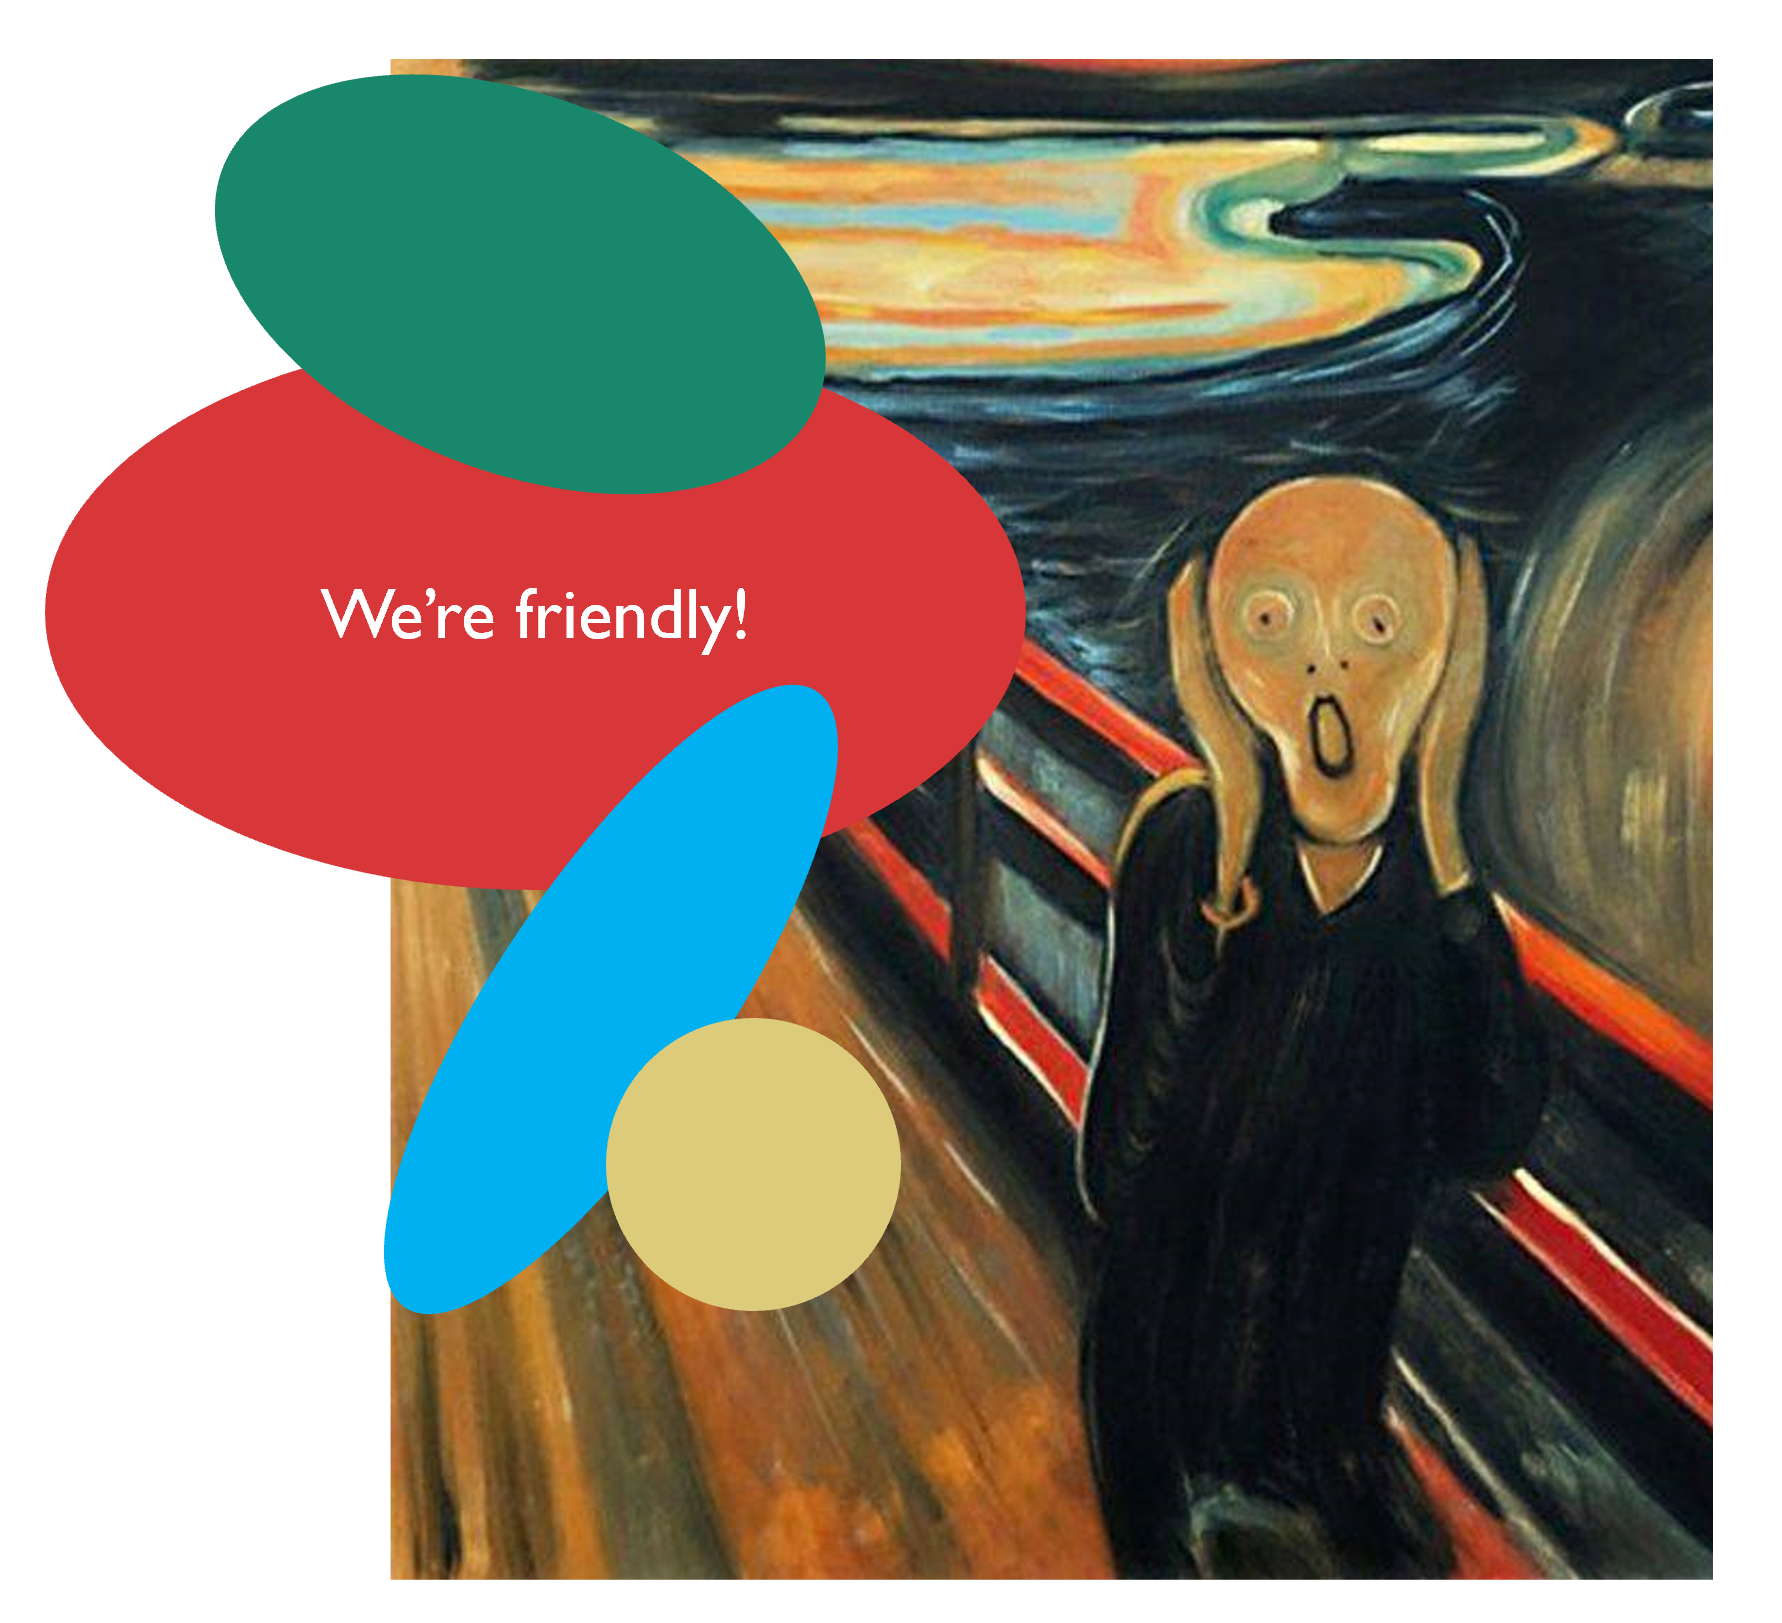
\includegraphics[height=.33\textwidth]{pics/0000_friendly_ellipses.png}}}
%  \end{picture}}

\author[Reznik, Garcia, Koiller]{}
\institute[]{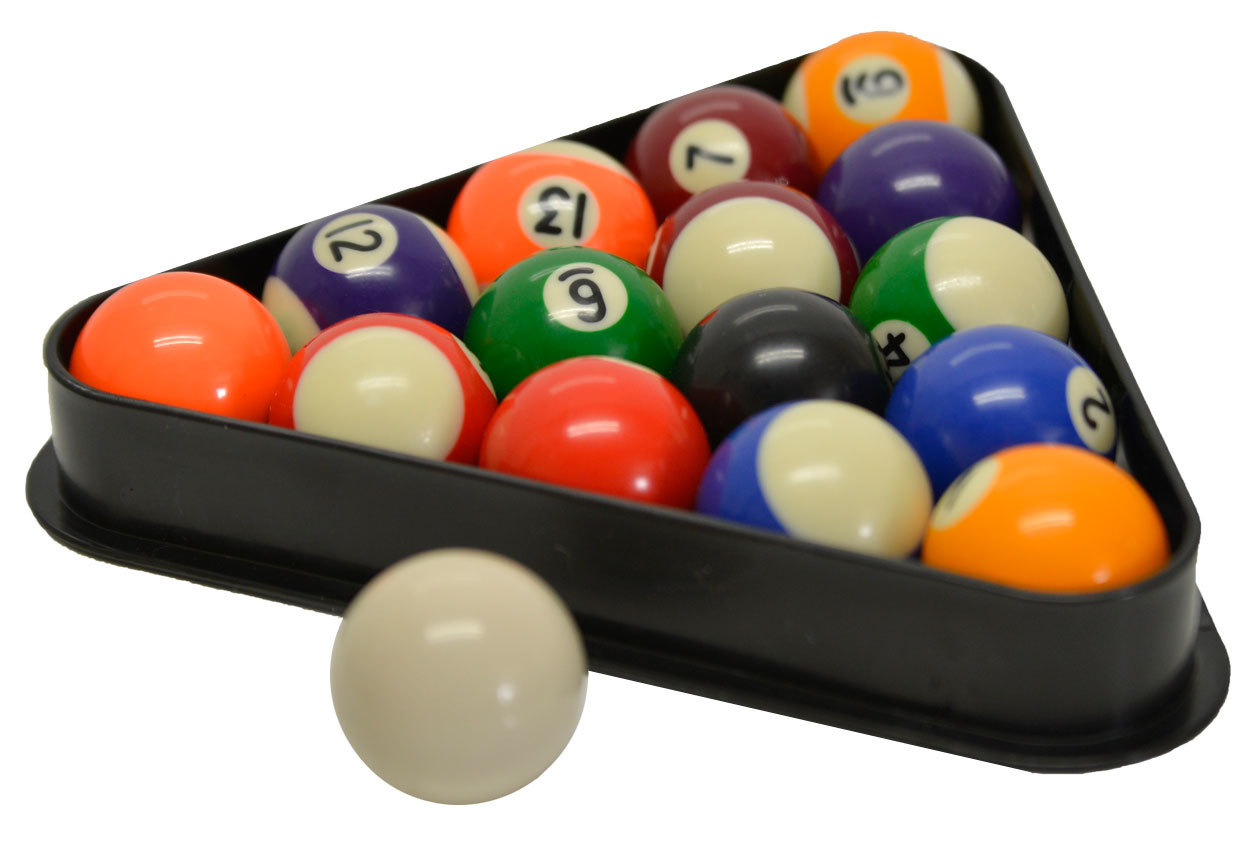
\includegraphics[height=.33\textheight]{pics/0000_billiard_rack.png}
%pics/0000_friendly_ellipses.png
\\[10pt] D. Reznik -- Upper West Soluções \and
R. Garcia -- Univ. Federal de Goiás \and 
J. Koiller -- Univ. Federal de Juiz de Fora}

\date{}


\begin{document}

\frame{\titlepage}
    
%\begin{frame}{Summary}
%\tableofcontents
%\end{frame}

\section{Preliminaries}
\frame{\sectionpage}
\begin{frame}{Billiard Trajectories \href{https://youtu.be/A7mPzrNJHkA}{[video]}}
\begin{figure}
    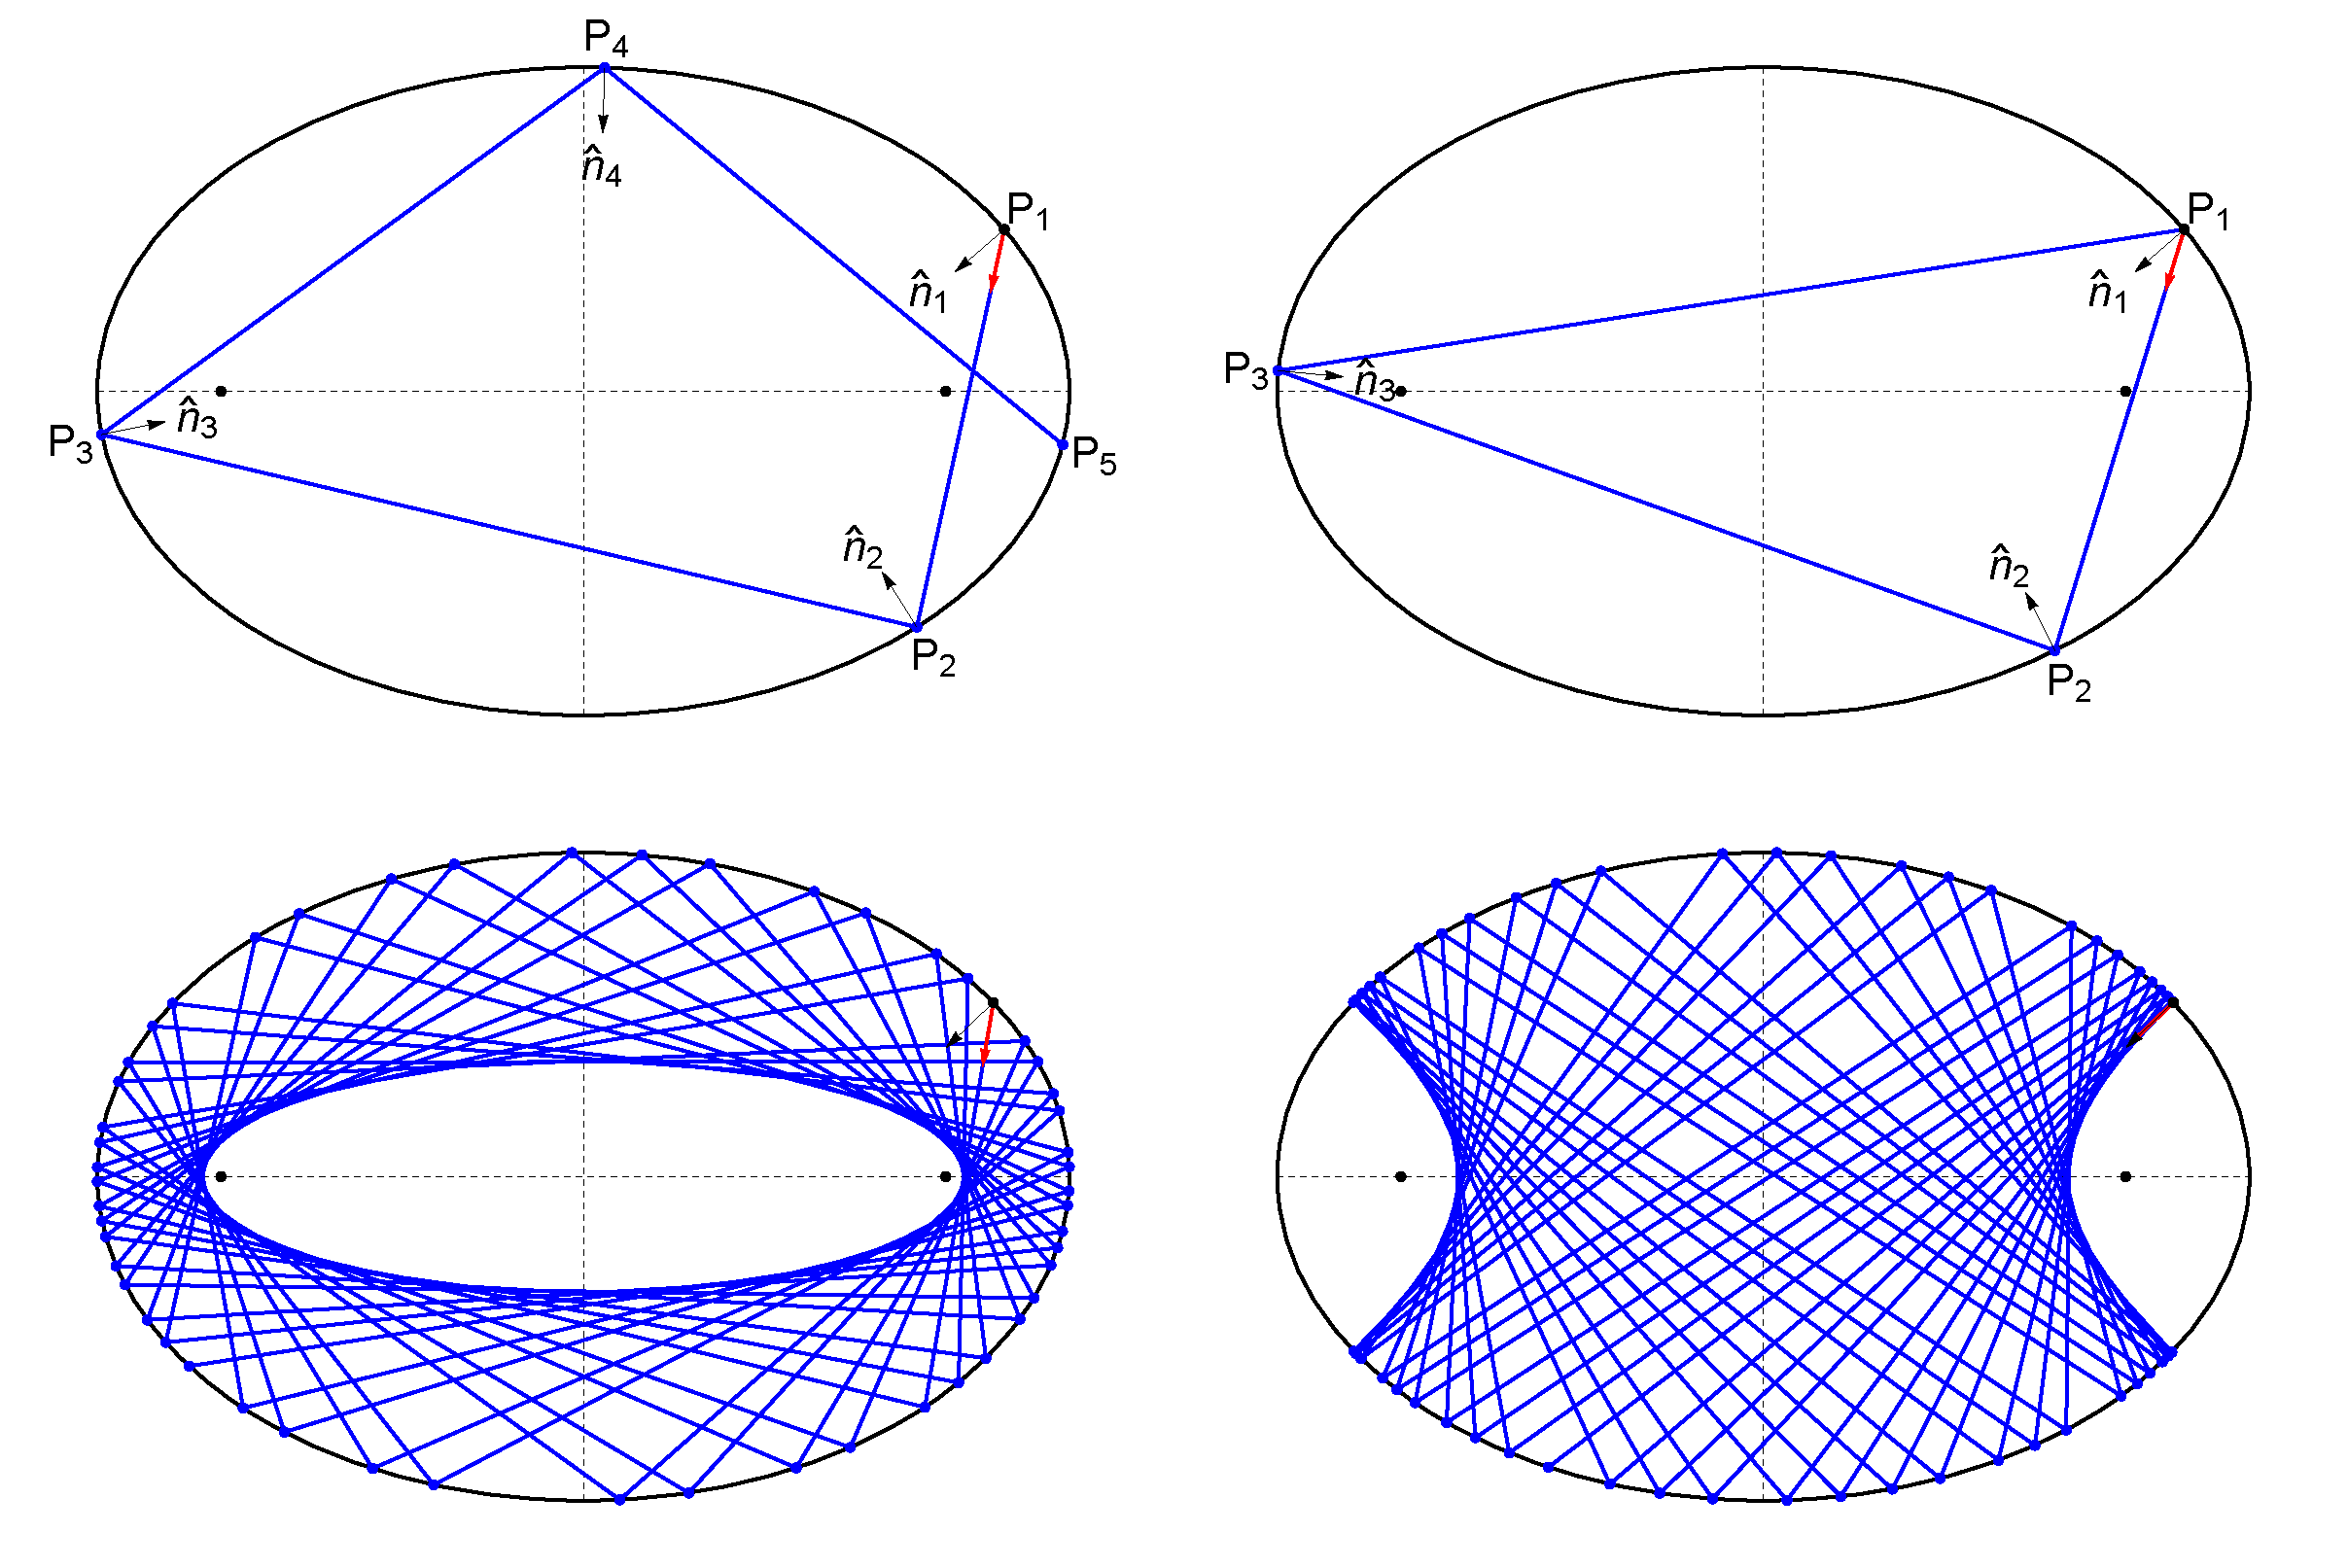
\includegraphics[height=.8\textheight]{pics/1000_billiard_trajectories.pdf}
\end{figure}
\end{frame}

\begin{frame}{Integrability \& Conservation}
\begin{figure}
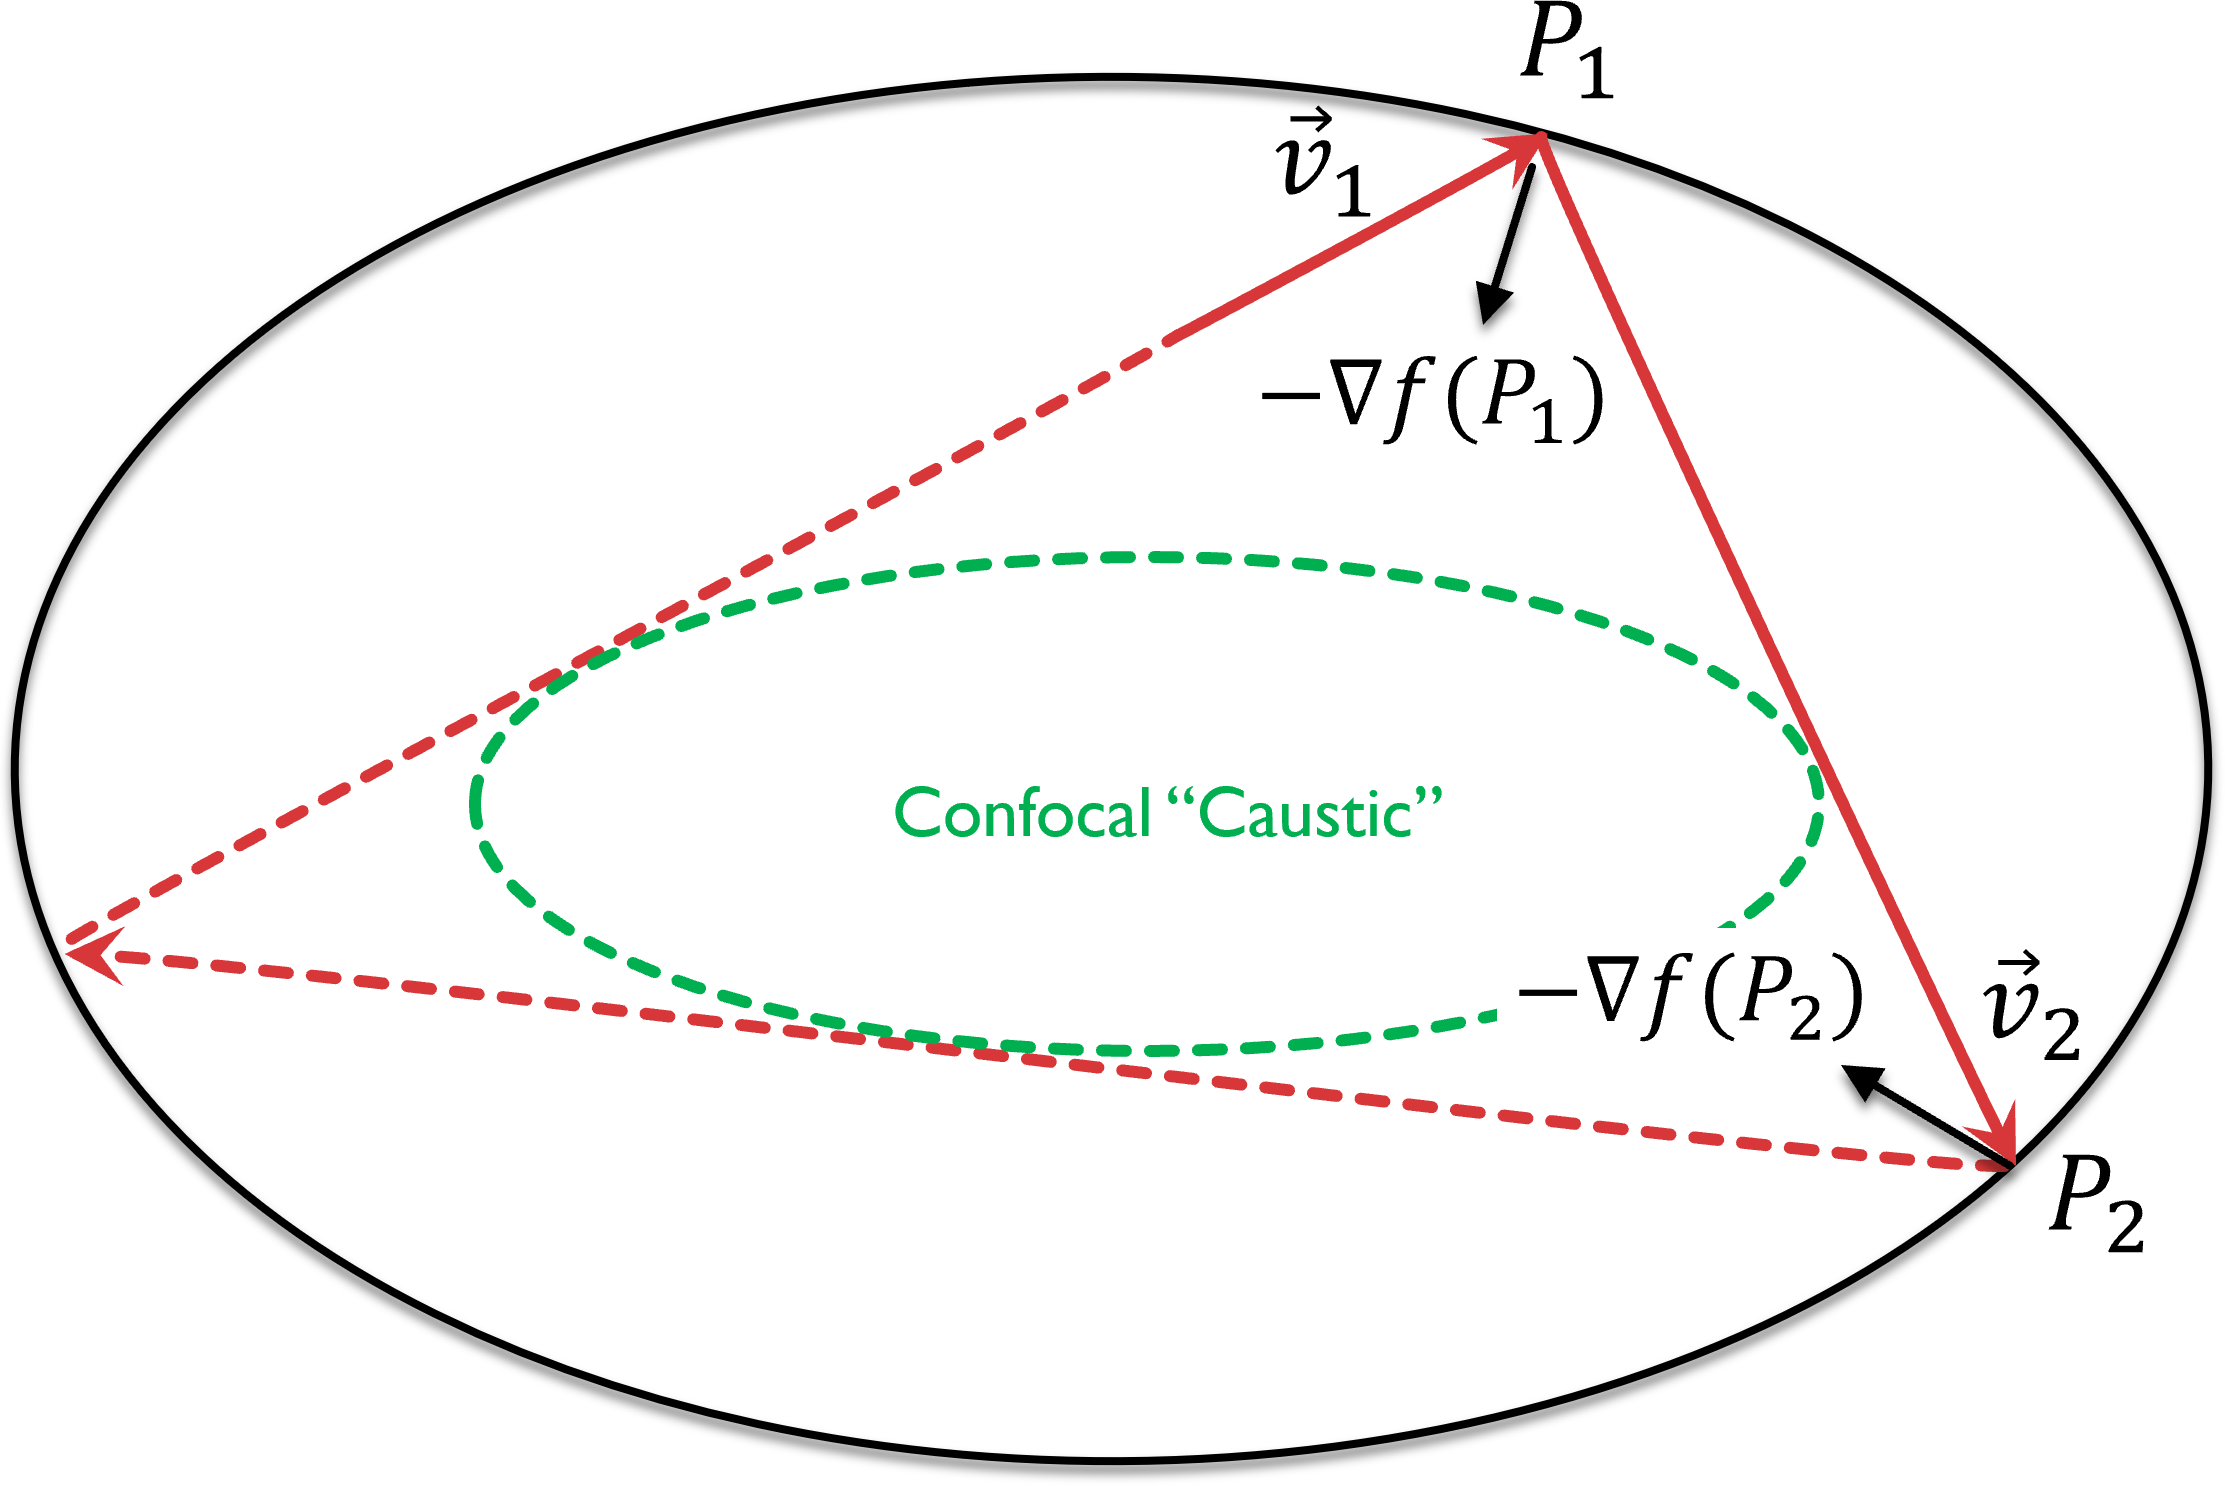
\includegraphics[height=.6\textheight]{pics/0000_integrability.png}
\end{figure}

\vspace*{-1cm}
\begin{align*}
\mbox{Energy} \implies L&=const.\\
\mbox{Joachmisthal's} \implies \gamma&=\frac{1}{2}\hat{v}.\nabla{f}(P)=const.
\end{align*}

\end{frame}

%\begin{frame}{Conservation: $L$ and $\gamma$}
%\begin{eqnarray*}
%f(x,y)&=&\left(\frac{x}{a}\right)^2+\left(\frac{y}{b}\right)^2=1 \\[10pt]
%\nabla{f}&=&2\left[\frac{x}{a^2},\frac{y}{b^2}\right]^t \\[10pt]
%\gamma&=&\frac{1}{2}\hat{v}.\nabla{f}(P)=\mbox{constant} >0,\,\,\,\forall{P}
%\end{eqnarray*}
%\end{frame}

\begin{frame}{$N=3$ Caustic \href{https://youtu.be/Y3q35DObfZU}{[video]}}
\begin{figure}
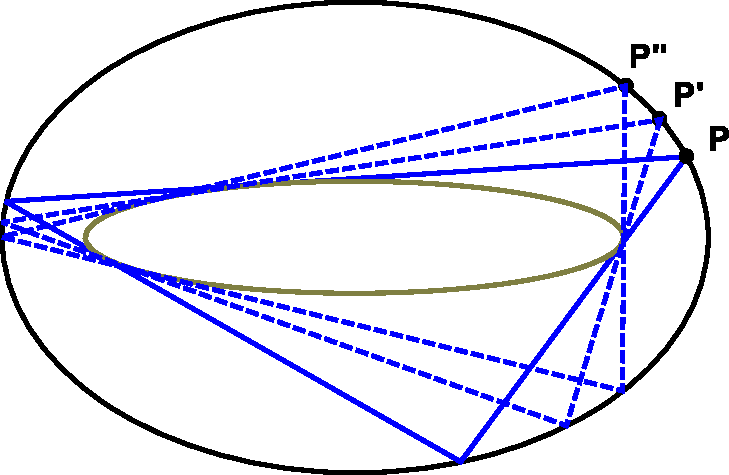
\includegraphics[height=.7\textheight]{pics/0010_three_orbits.pdf}
\end{figure}
\end{frame}

\begin{frame}{Poncelet's Porism}
\begin{figure}
    \centering
    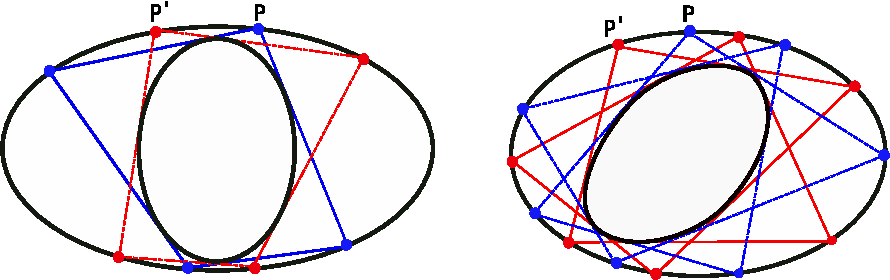
\includegraphics[width=\textwidth]{pics/0003_poncelet_porism.pdf}
\end{figure}
\end{frame}



%\section{Preliminaries: Integrability and Conservation}
%\frame{\sectionpage}
%\input{01a_integrability}

\section{Locus Pocus}
\frame{\sectionpage}
\begin{frame}{Triangle Geometry}

\begin{minipage}[c]{0.85\textwidth}
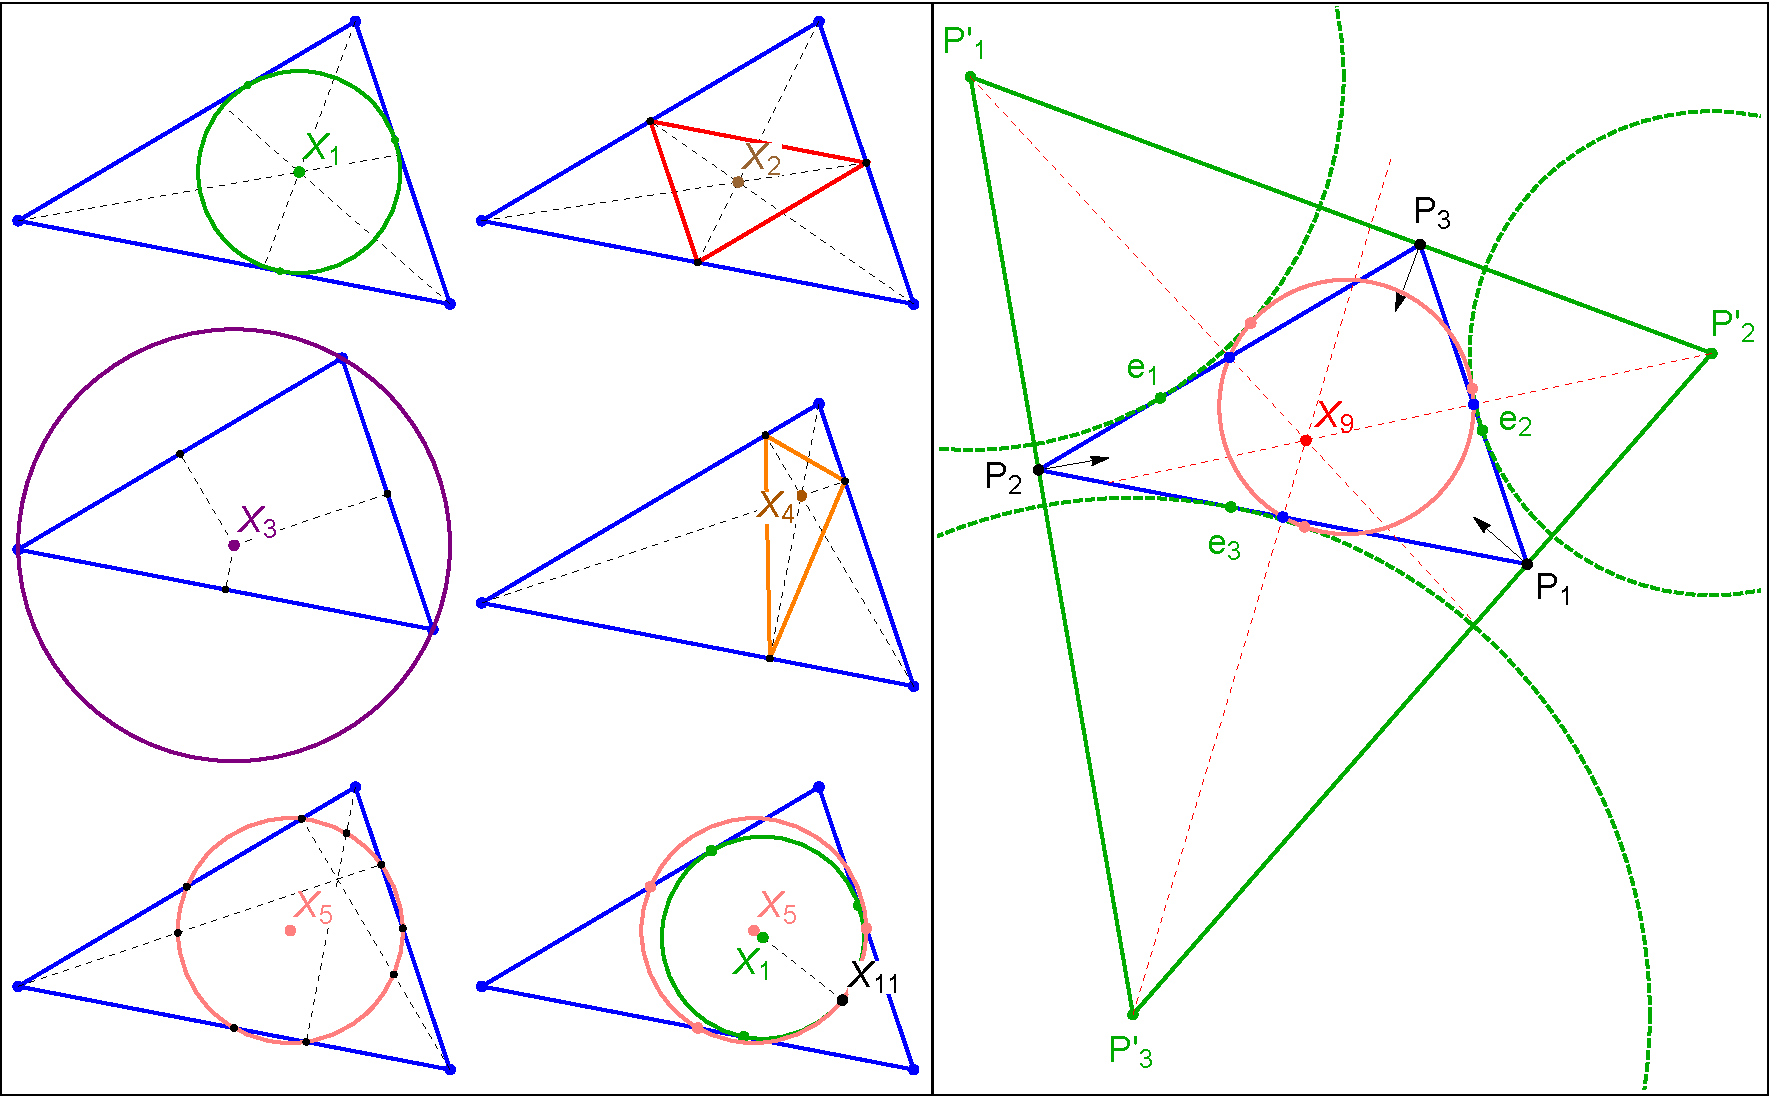
\includegraphics[width=.85\textwidth]{pics/0039_constr.pdf}
\end{minipage}
\hspace{-1.5cm}
\begin{minipage}[c]{.2\textwidth}
\begin{table}
\tiny
\begin{tabular}{p{1em}l}
$X_1$ & Incenter \\
$X_2$ & Barycenter \\
$X_3$ & Circumcenter \\
$X_4$ & Orthocenter \\
$X_5$ & 9-Point center \\
$X_9$ & Mittenpunkt \\
$X_{11}$ & Feuerbach Point
\end{tabular}
\end{table}
\end{minipage}
\end{frame}

\begin{frame}{Locus of Incenter is Elliptic \href{https://www.youtube.com/watch?v=BBsyM7RnswA}{[video]}}
\begin{figure}
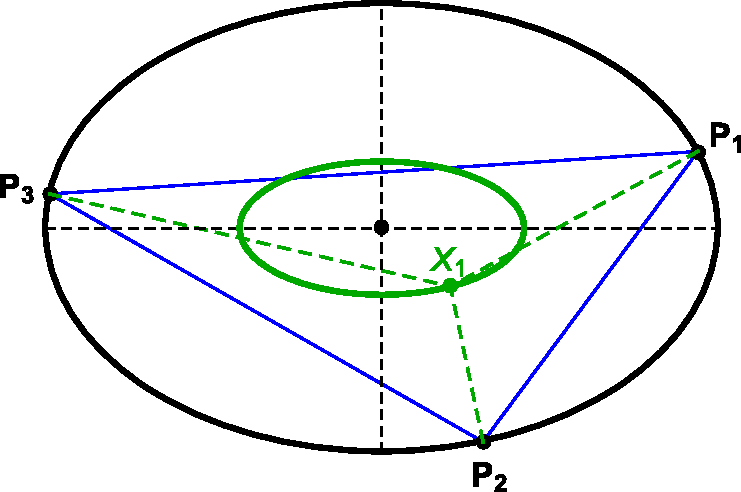
\includegraphics[height=.7\textheight]{pics/0020_incenter_locus.pdf}
\end{figure}
\end{frame}

\begin{frame}{Locus Intouch Points is Sextic \href{https://youtu.be/9xU6T7hQMzs}{[video]}}
\begin{figure}
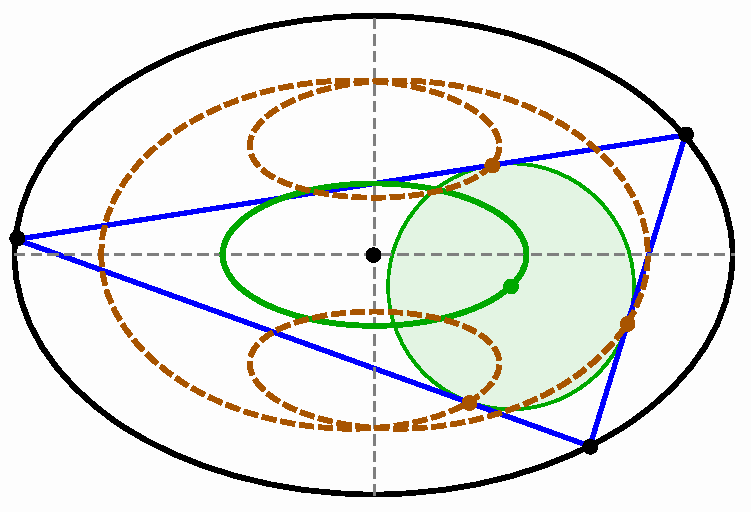
\includegraphics[height=.7\textheight]{pics/0001_intro_plot.pdf}
\end{figure}
\end{frame}

\begin{frame}{Interactive \href{https://editor.p5js.org/undefined/present/i1Lin7lt7}{Applet}}
\begin{figure}
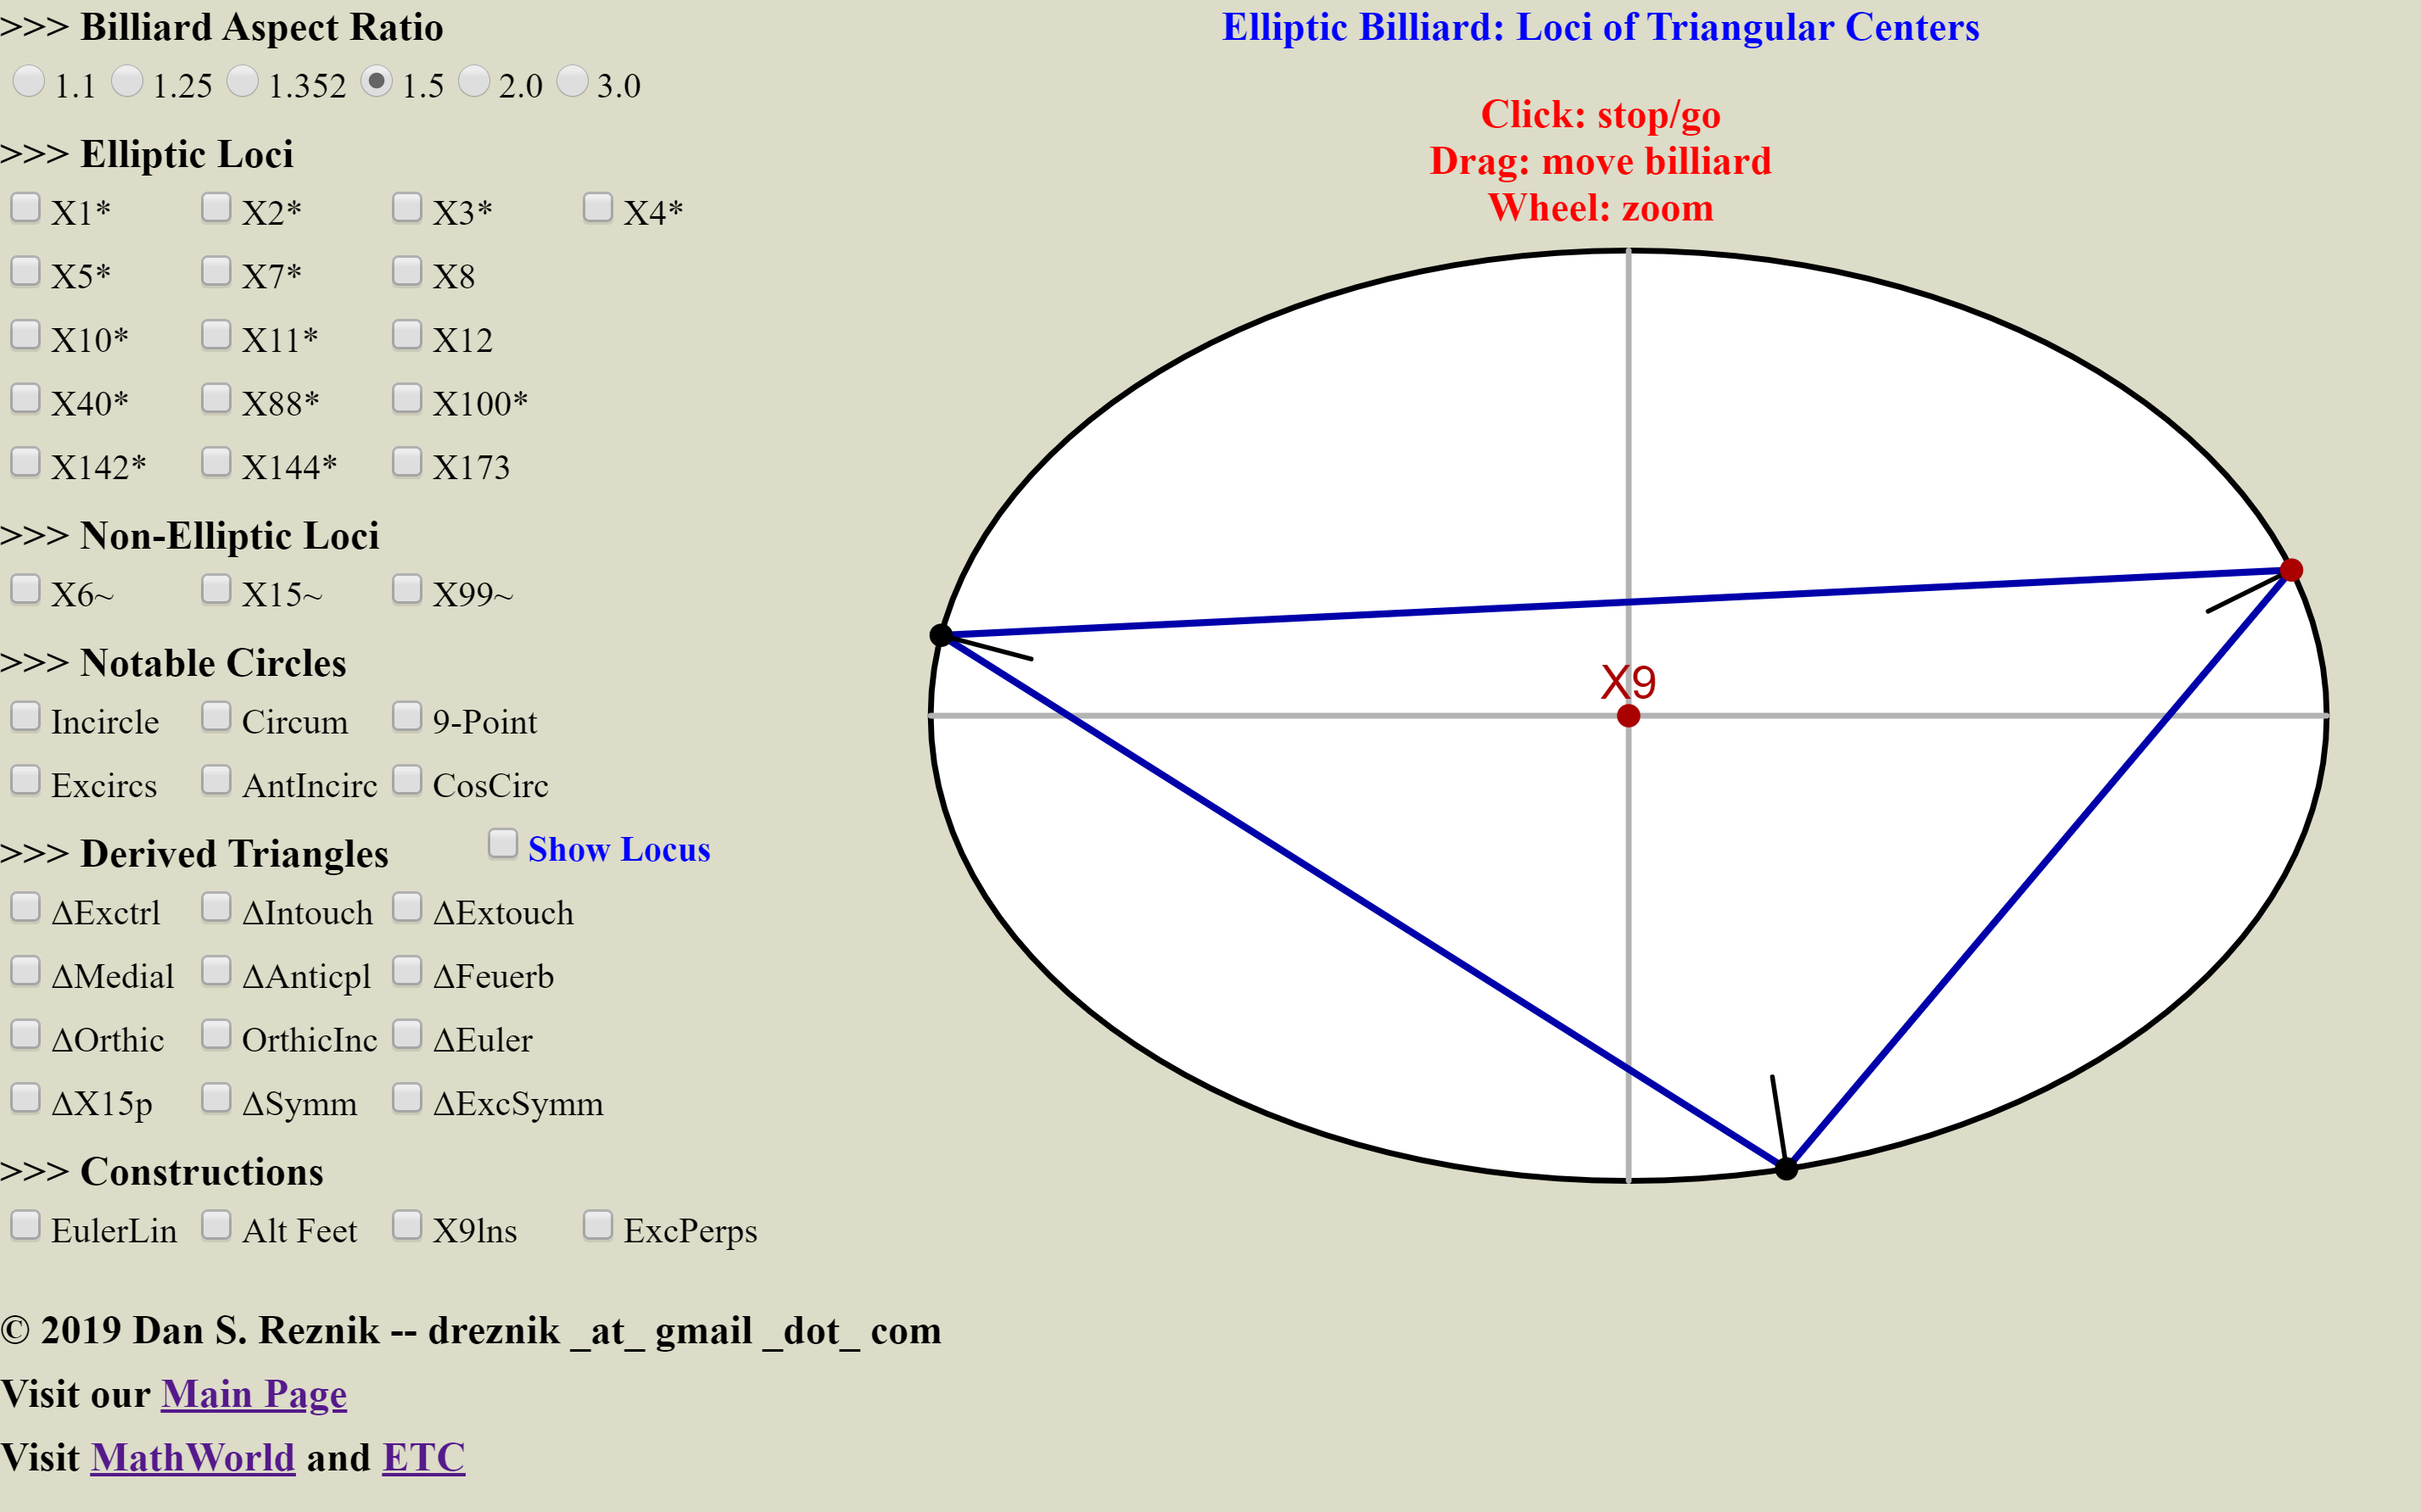
\includegraphics[height=.8\textheight]{pics/applet_p5js.png}
\end{figure}
\end{frame}  

\begin{frame}{Locus of Excenters is Elliptic \href{https://youtu.be/Xxr1DUo19_w}{[video]}}
\begin{figure}
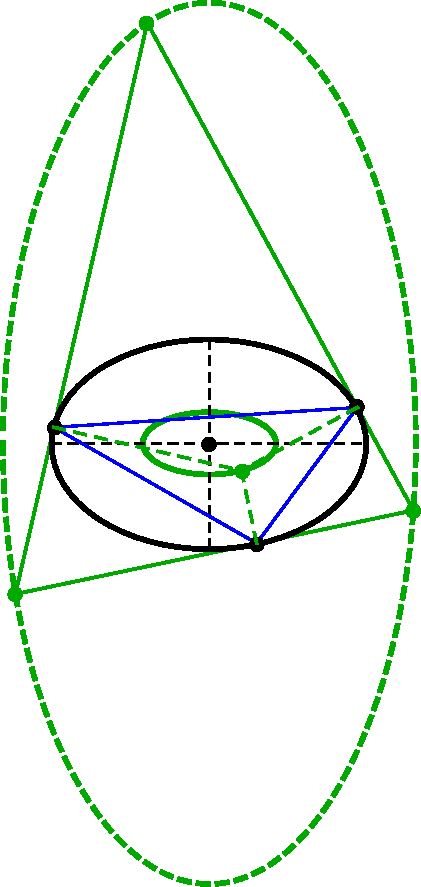
\includegraphics[clip,trim={0 4cm 0 0},height=.8\textheight]{pics/0025_incenter_excenter_locus.pdf}
\end{figure}
\end{frame}

%\begin{frame}{Major Triangular Centers}
%\begin{figure}
%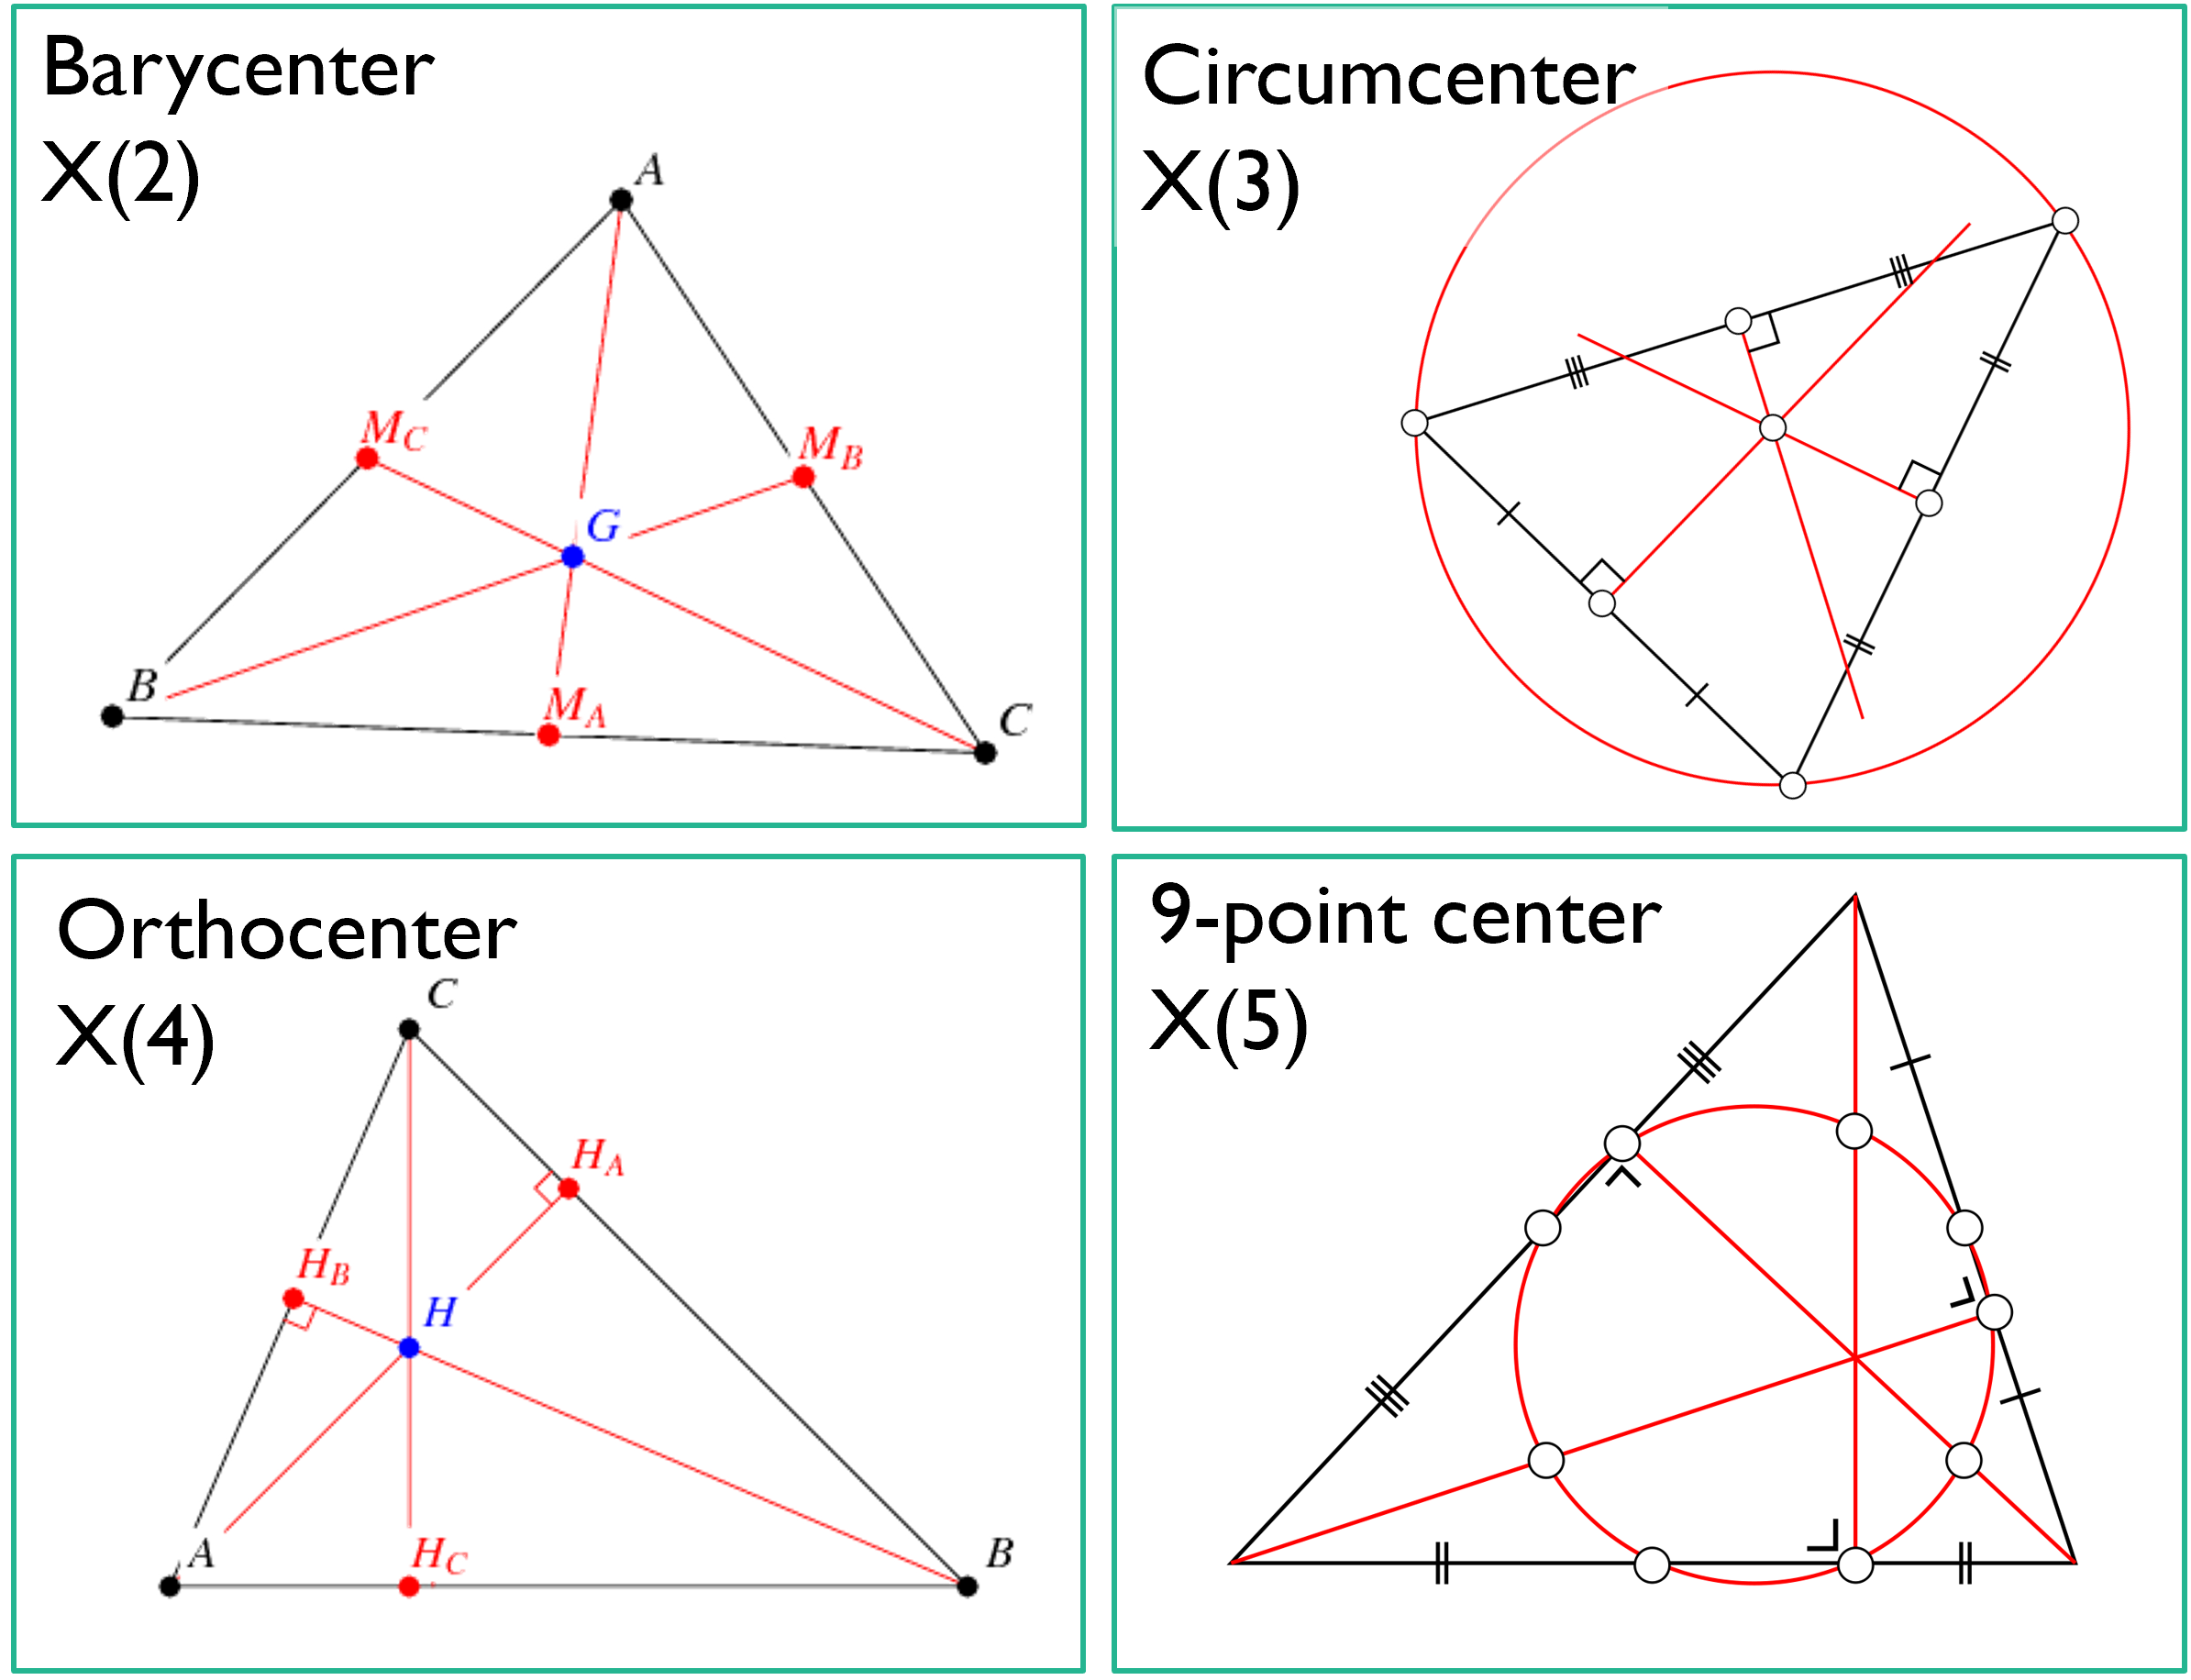
\includegraphics[height=.8\textheight]{pics/0000_major_centers.png}
%\end{figure}
%\end{frame}

\begin{frame}{Encyclopedia of Triangular Centers \href{https://faculty.evansville.edu/ck6/encyclopedia/ETC.html}{[ETC]}}
\begin{figure}
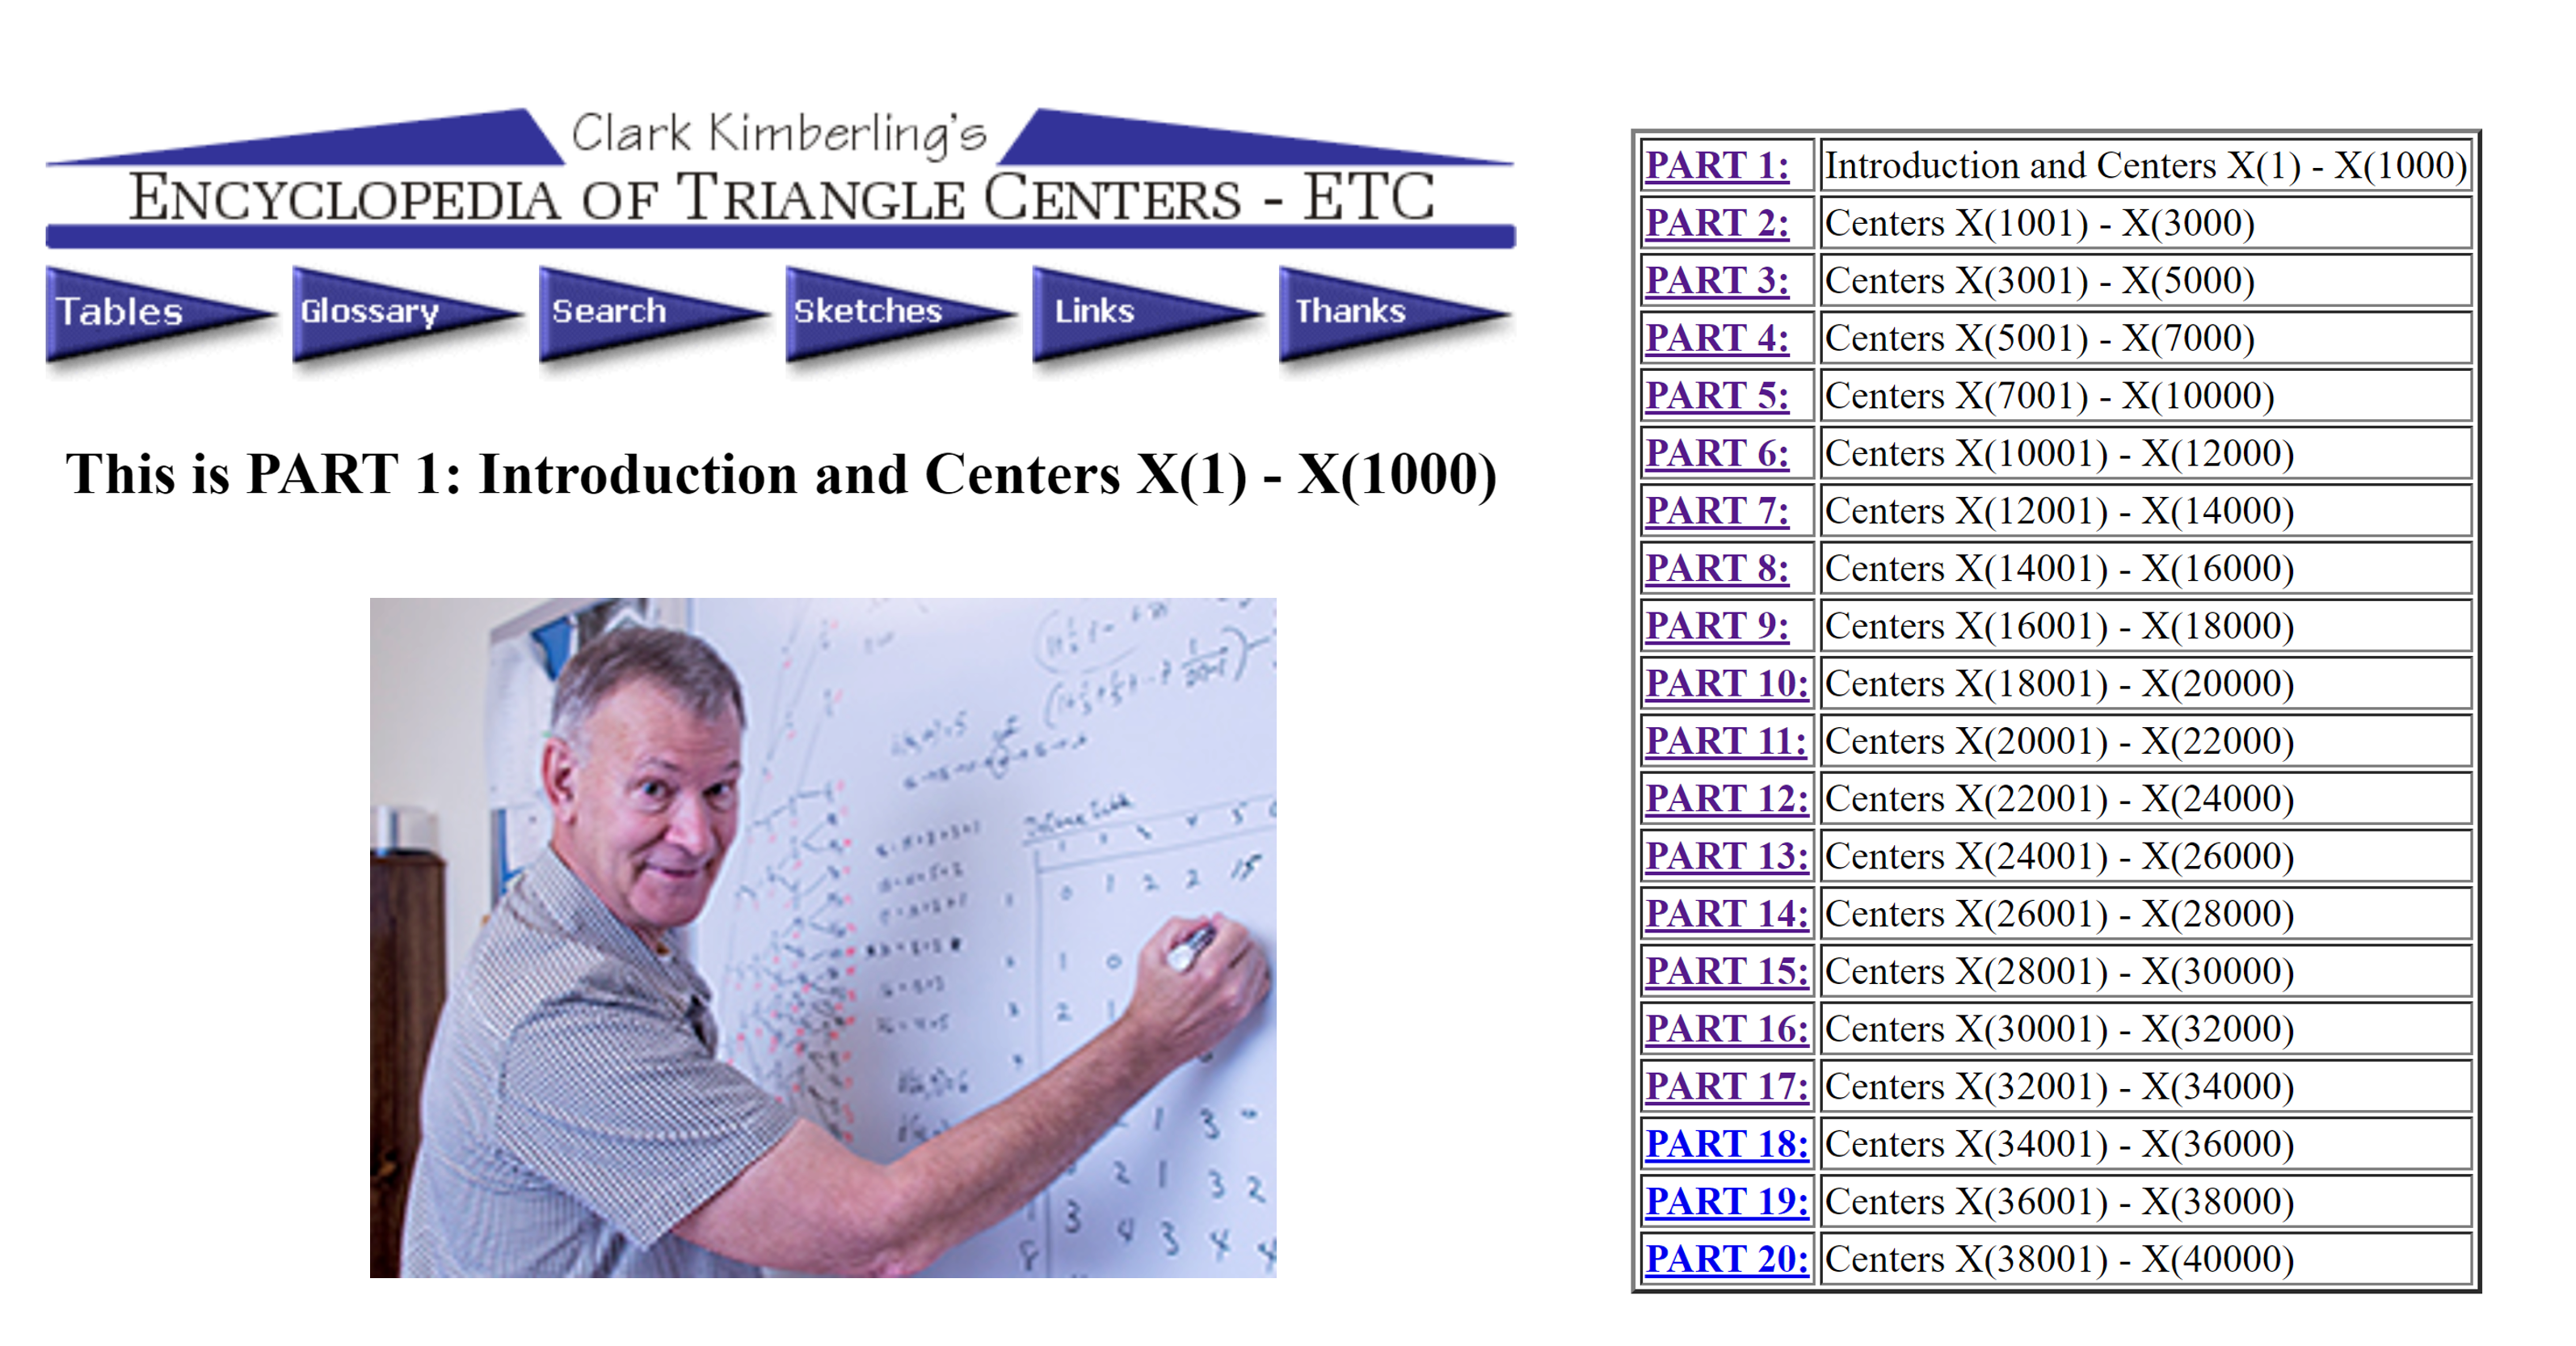
\includegraphics[height=.8\textheight]{pics/0000_etc.png}
\end{figure}
\end{frame}

\begin{frame}{Elliptic Loci of Major Triangular Centers \href{https://youtu.be/sMcNzcYaqtg}{[video]}}
\begin{figure}
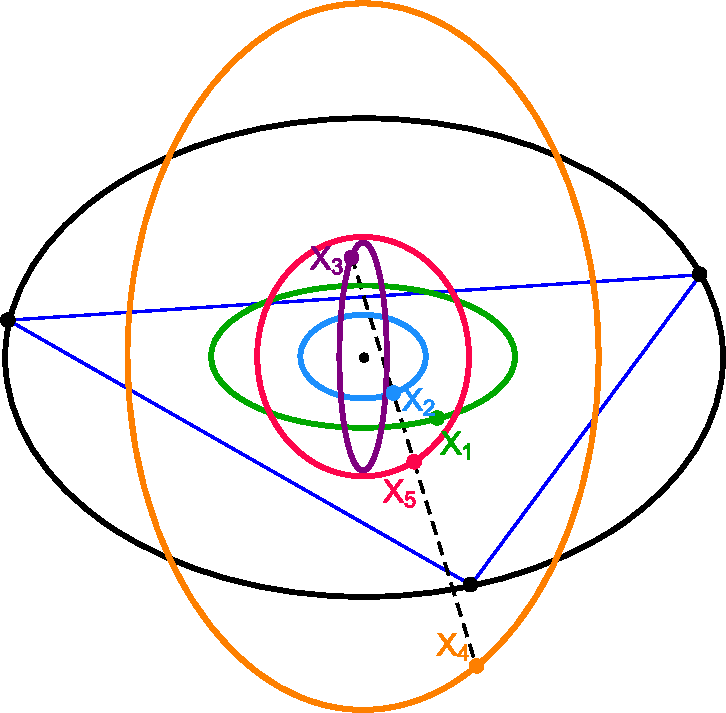
\includegraphics[height=.75\textheight]{pics/0030_x12345_locus.pdf}
\end{figure}
\end{frame}

\begin{frame}{Derived Triangles \href{https://youtu.be/xyroRTEVNDc}{[video]}}
\begin{figure}
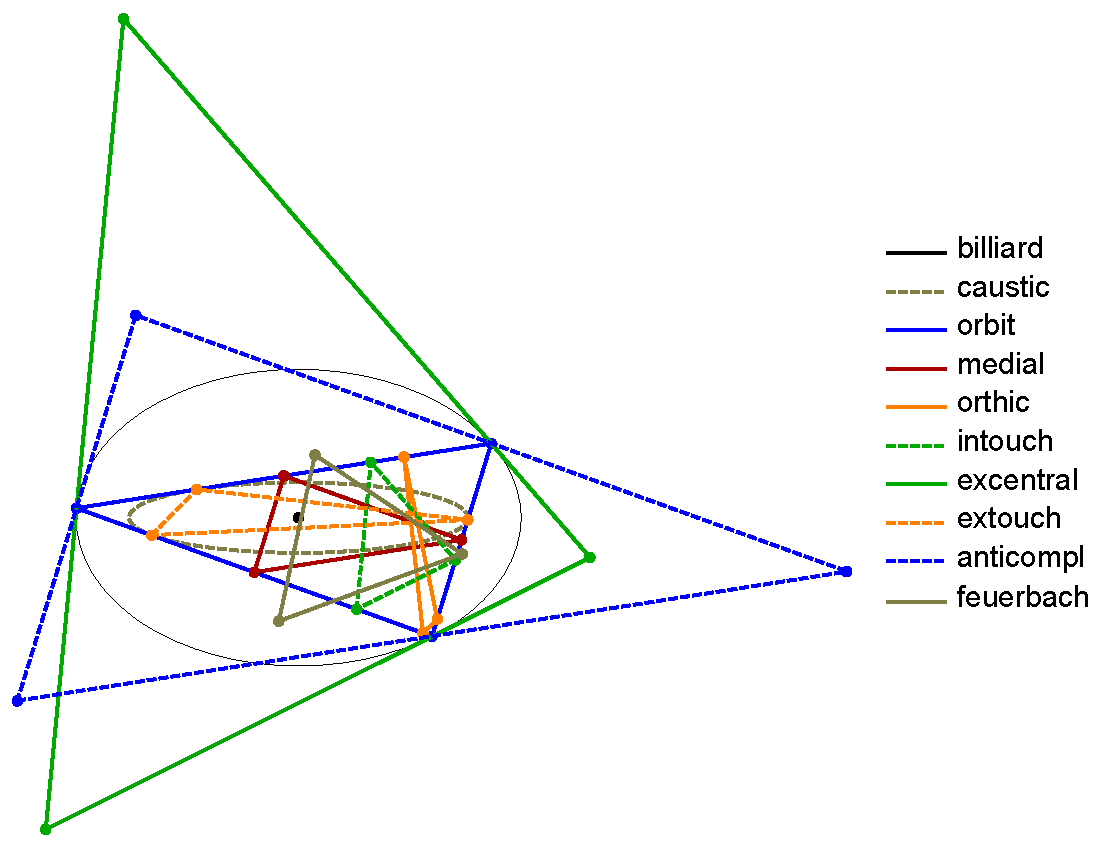
\includegraphics[clip,trim={0 0 0 3cm},height=.8\textheight]{pics/0043_derived-triangles.pdf}
\end{figure}
\end{frame}

\begin{frame}{Loci of Vertices of Derived Triangles \href{https://youtu.be/OGvCQbYqJyI}{[video]}}
\begin{figure}
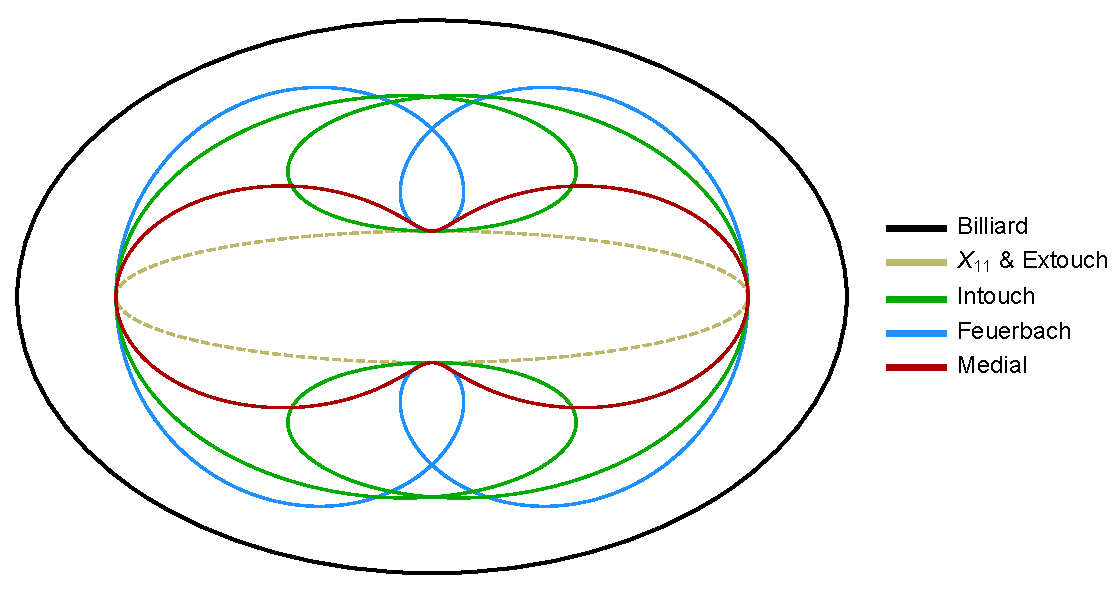
\includegraphics[height=.7\textheight]{pics/0040_non_elliptic.pdf}
\end{figure}
\end{frame}

\begin{frame}{Feuerbach, Anticomplement, and Extouchpoints \href{https://youtu.be/TXdg7tUl8lc}{[video]}}
\begin{figure}
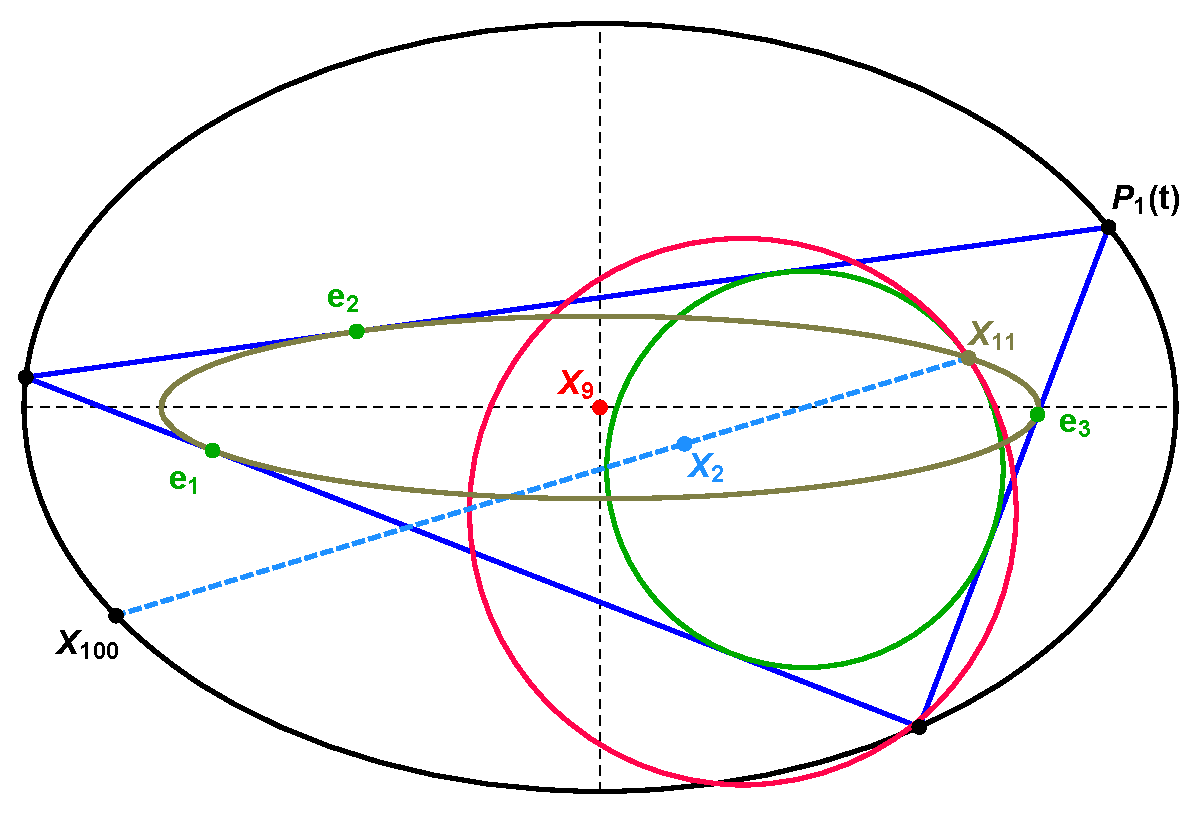
\includegraphics[height=.75\textheight]{pics/0035_feuerbach_loci.pdf}
\end{figure}
\end{frame}

\begin{frame}{Symmedian Point: Quasi-Elliptic Convex Quartic}
\begin{tabular}{rl}    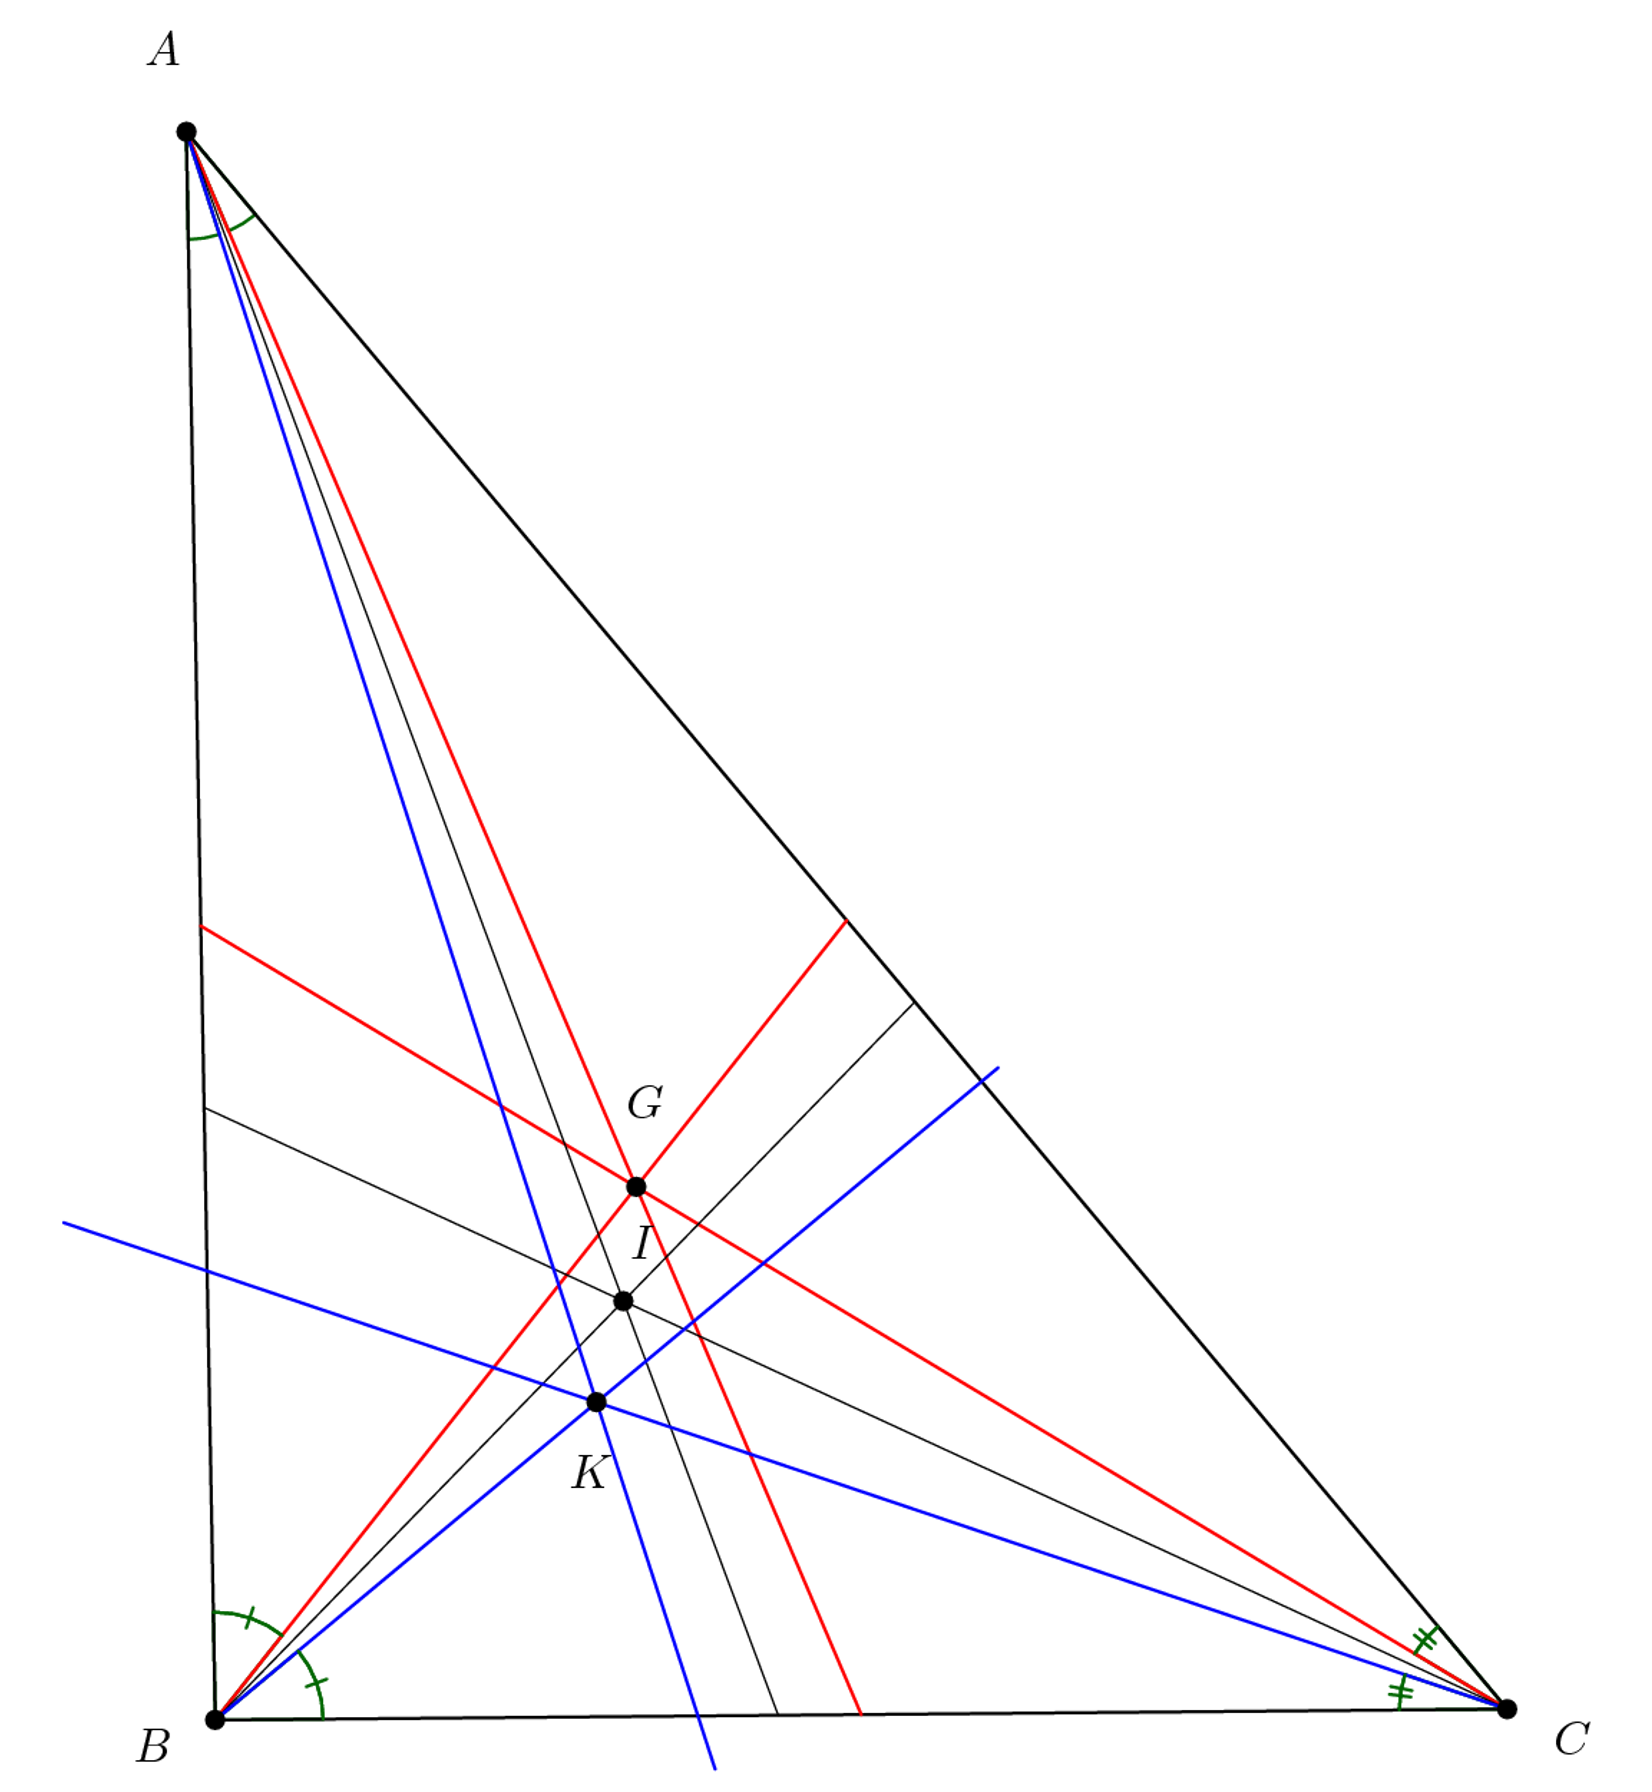
\includegraphics[width=.4\textwidth]{pics/0000_symmedian.png} & \hspace{-1cm} 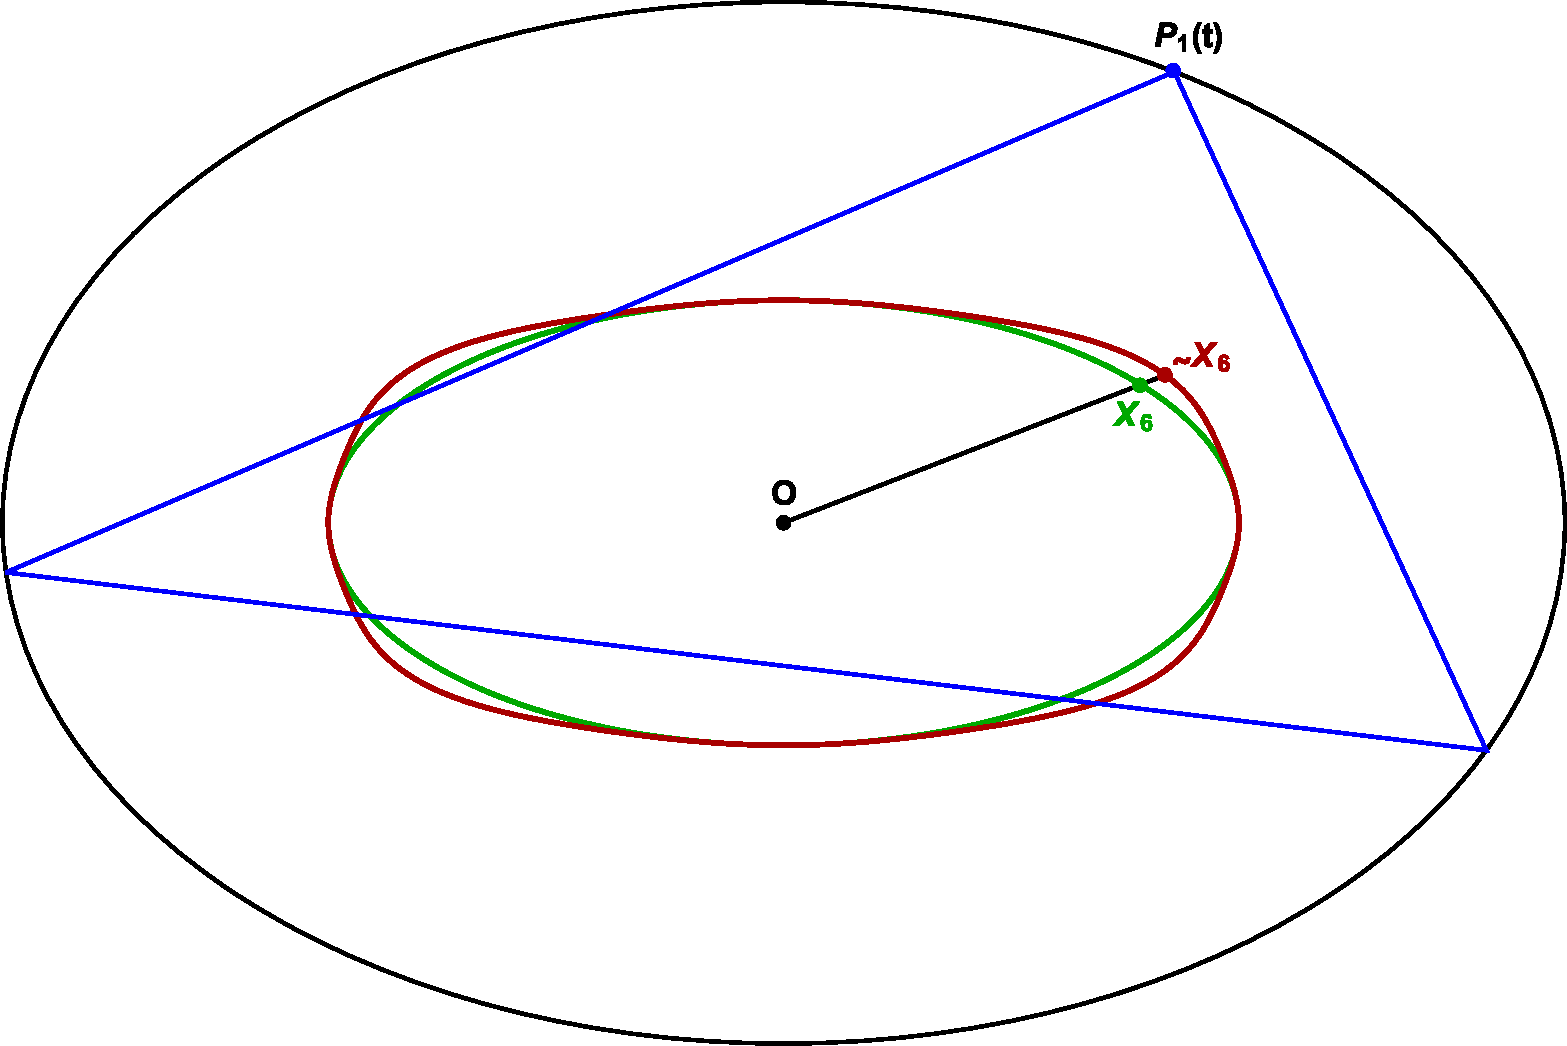
\includegraphics[width=.6\textwidth]{pics/0041_symmedian.pdf}
\end{tabular}
\end{frame}

\begin{frame}{Orthic Incenter: Four Kinks \href{https://youtu.be/3qJnwpFkUFQ}{[video]}}
\begin{figure}
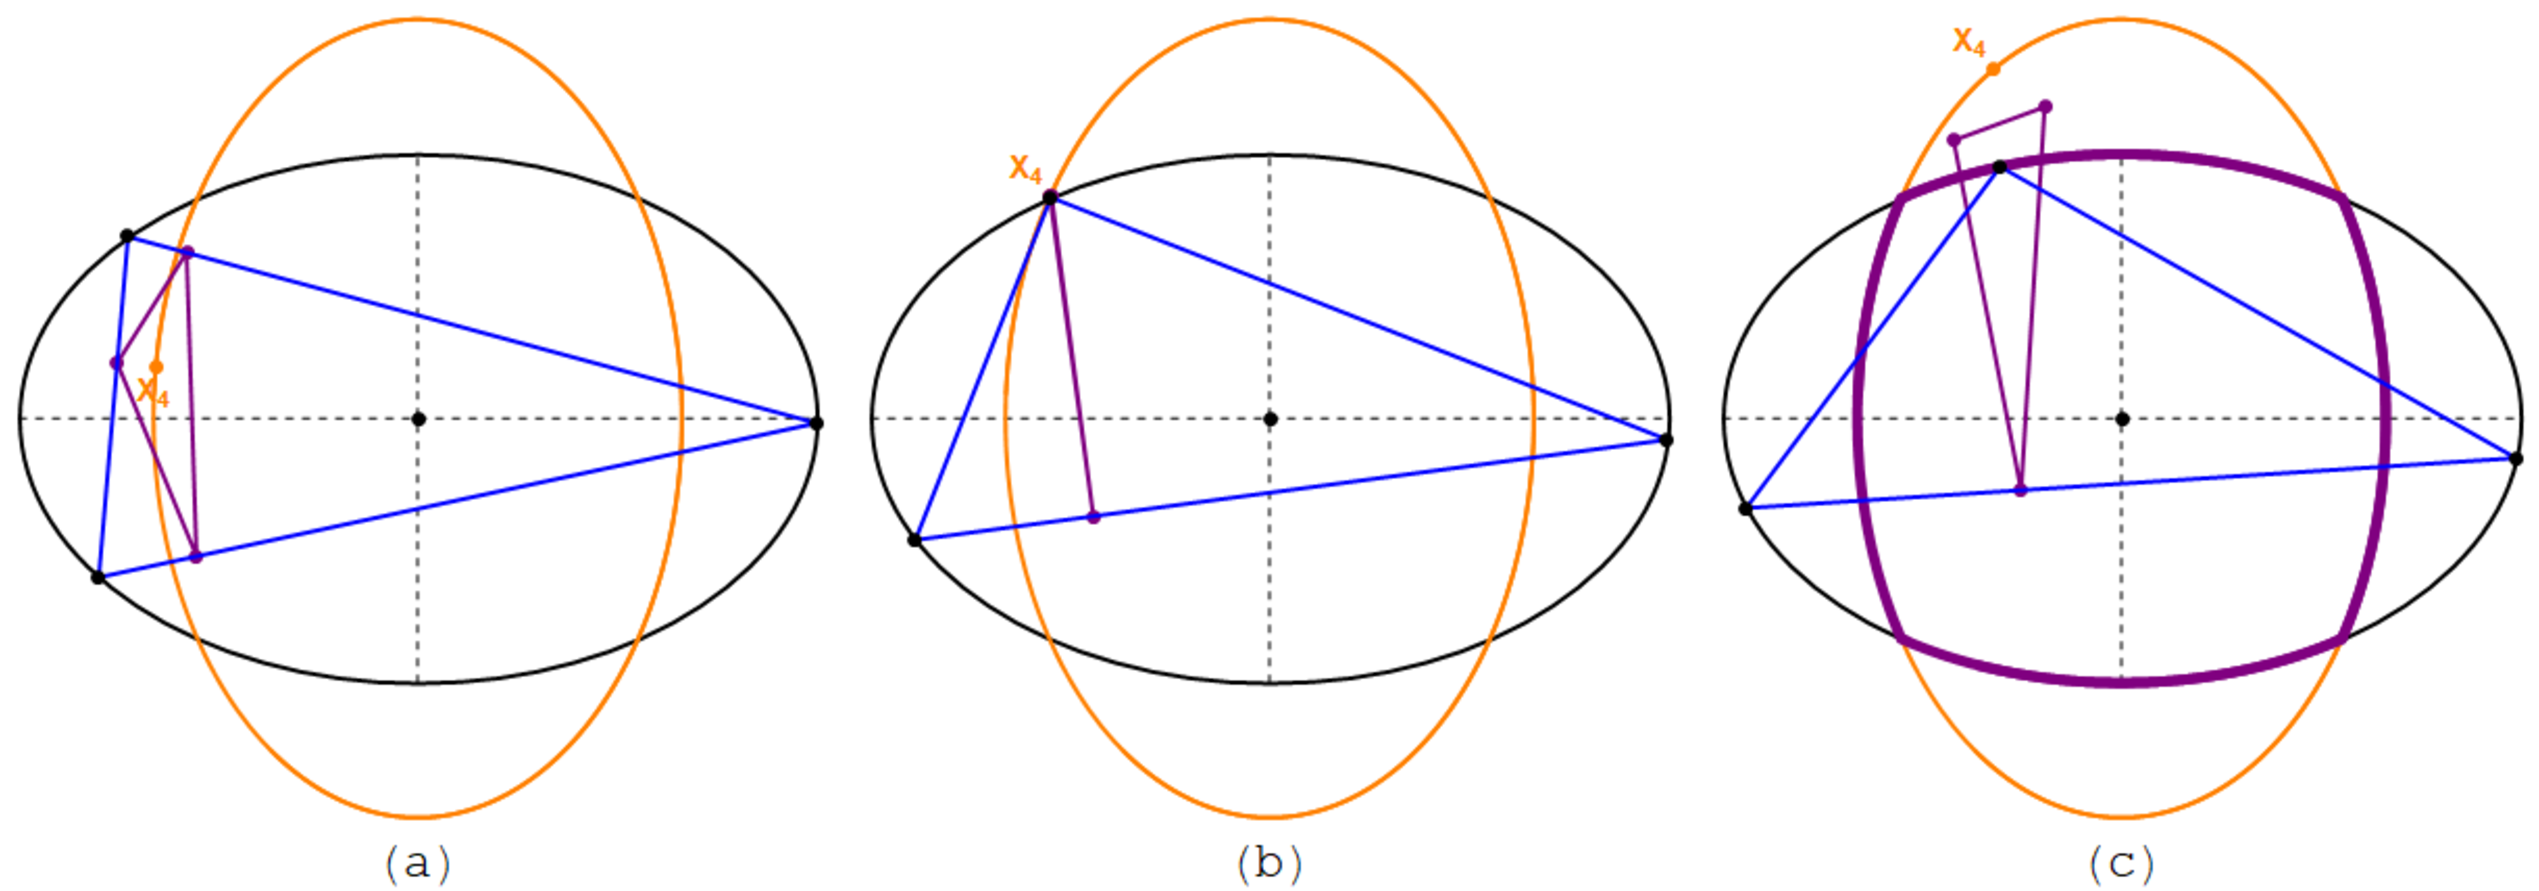
\includegraphics[width=\textwidth]{pics/0045_ort_loci_orthic.pdf}
\end{figure}
\end{frame}

\begin{frame}{Intouchpoints of Anticomplementary Track Billiard \href{https://youtu.be/50dyxWJhfN4}{[video]}}
\begin{figure}
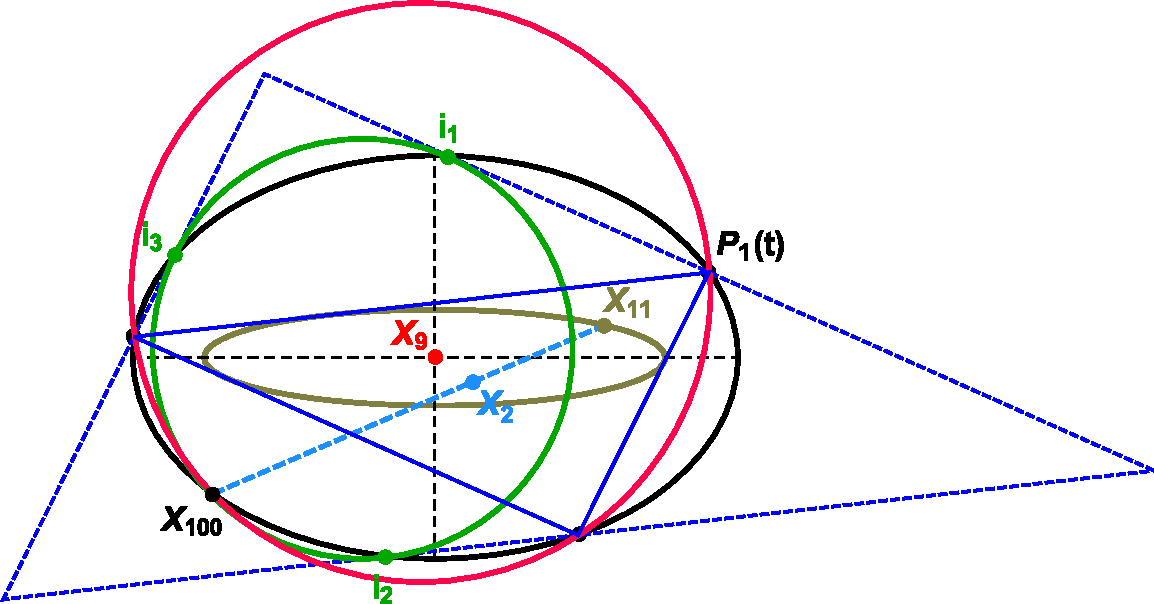
\includegraphics[height=.7\textheight]{pics/0048_act_intouch.pdf}
\end{figure}
\end{frame}

\begin{frame}{A Circular Locus! \href{https://youtu.be/hCQIT6_XhaQ}{[video]}}
\begin{tabular}{rl}
\begin{tabular}{r}
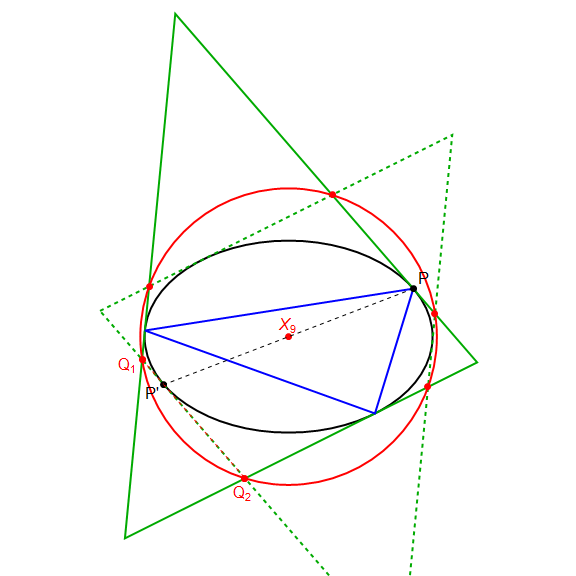
\includegraphics[height=.8\textheight]{pics/0120_cosine_circle_reflected_excentral.png}
\end{tabular} & \hspace{-1cm}\begin{tabular}{l}
\parbox{0.5\linewidth}{
  \begin{minipage}{0.45\textwidth}
  $$r^* = \frac{1}{\gamma}$$ \end{minipage}}
\end{tabular}  \\
\end{tabular}
\end{frame}

\section{A {\em Point} Locus!}
\frame{\sectionpage}
\begin{frame}{Mittenpunkt is Stationary  \href{https://youtu.be/tMrBqfRBYik}{[video]}}
\begin{figure}
\centering
     \begin{subfigure}[t]{0.45\textwidth}
         \centering
         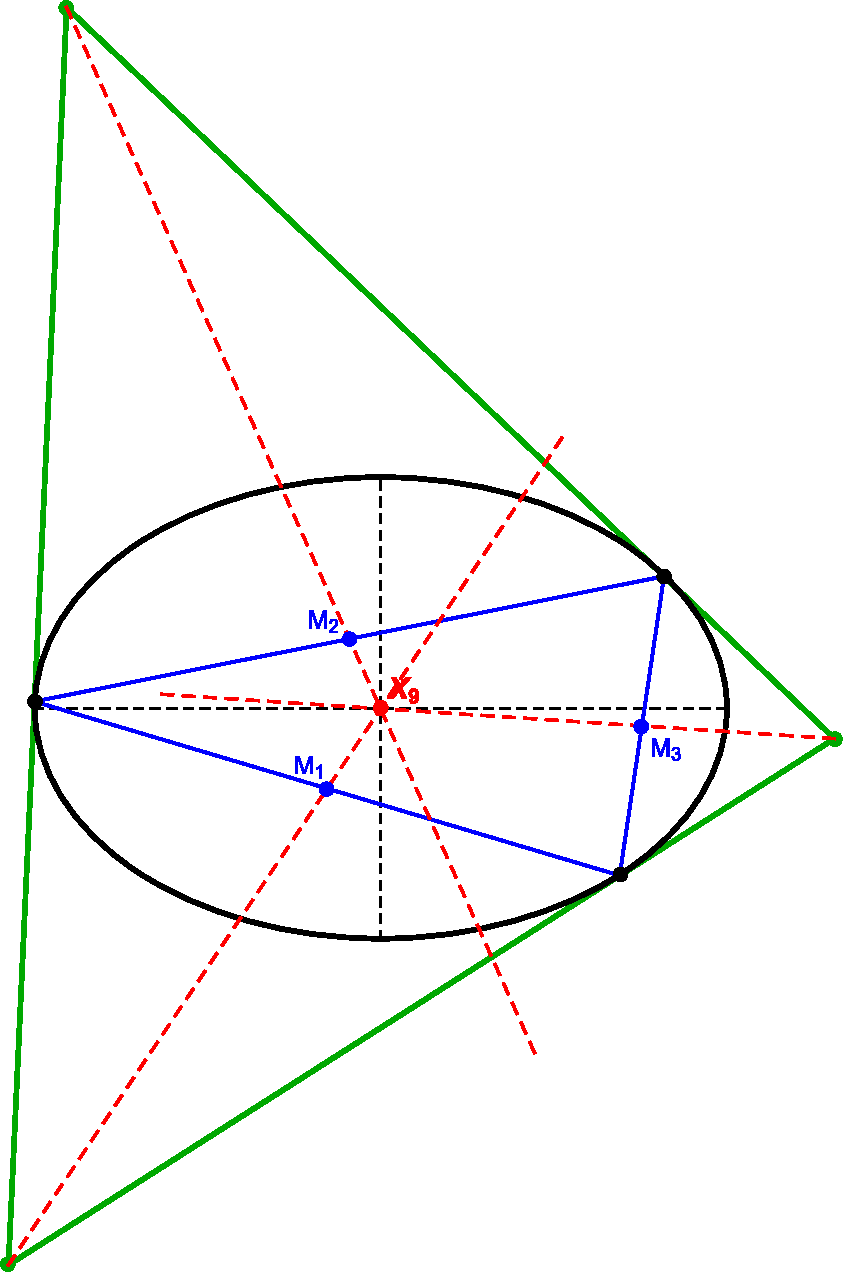
\includegraphics[height=.8\textheight]{pics/0052_mitten_rot.pdf}
     \end{subfigure}
     \hspace{-.5em}
     \begin{subfigure}[t]{0.45\textwidth}
         \centering
         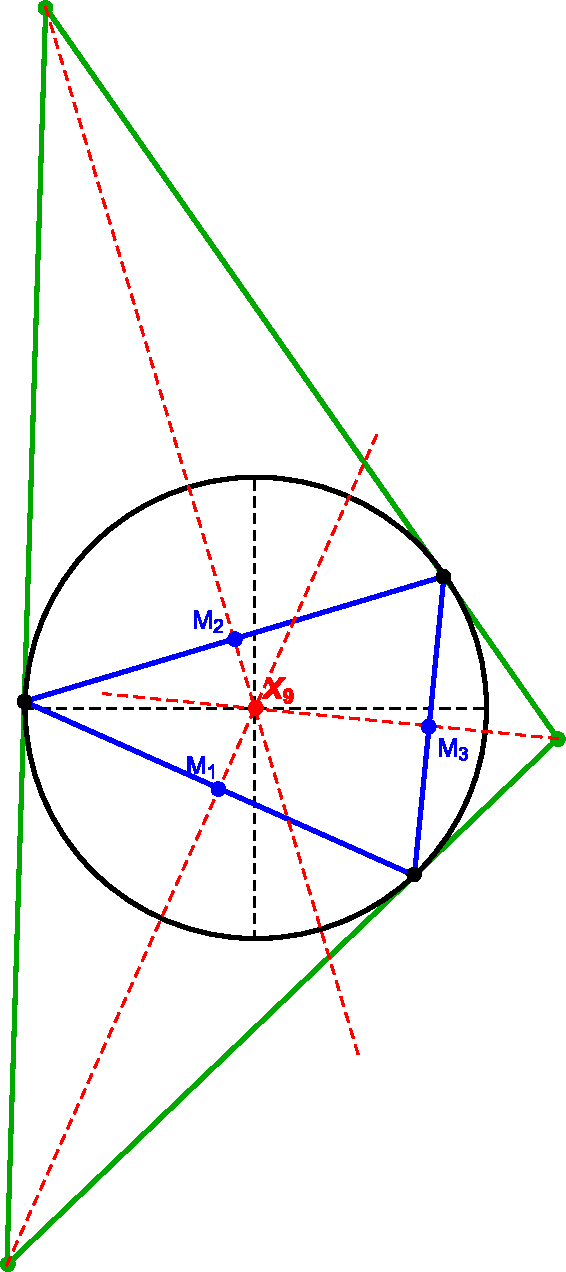
\includegraphics[height=.8\textheight]{pics/0053_mitten_rot_scaled.pdf}
     \end{subfigure}
\end{figure}
\end{frame}

\begin{frame}{Circumbilliard \href{https://youtu.be/vSCnorIJ2X8}{[video]}}
\begin{figure}
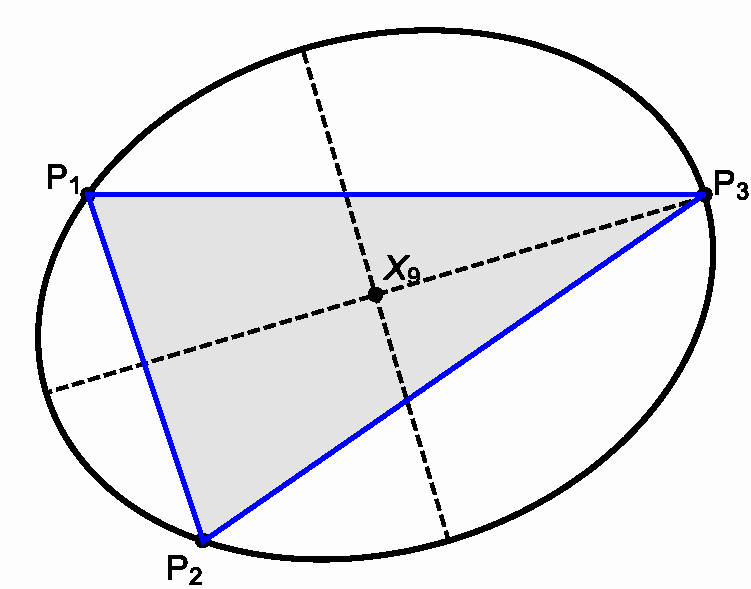
\includegraphics[height=.7\textheight]{pics/0056_circumplot.pdf}
\end{figure}
\end{frame}

%\section{A Circular Locus}
%\frame{\sectionpage}
%



\section{The Beautiful Ratio}
\frame{\sectionpage}
\begin{frame}{Three Little Radii \href{https://youtu.be/kxiC19ZrOVA}{[video]}}
\begin{figure}
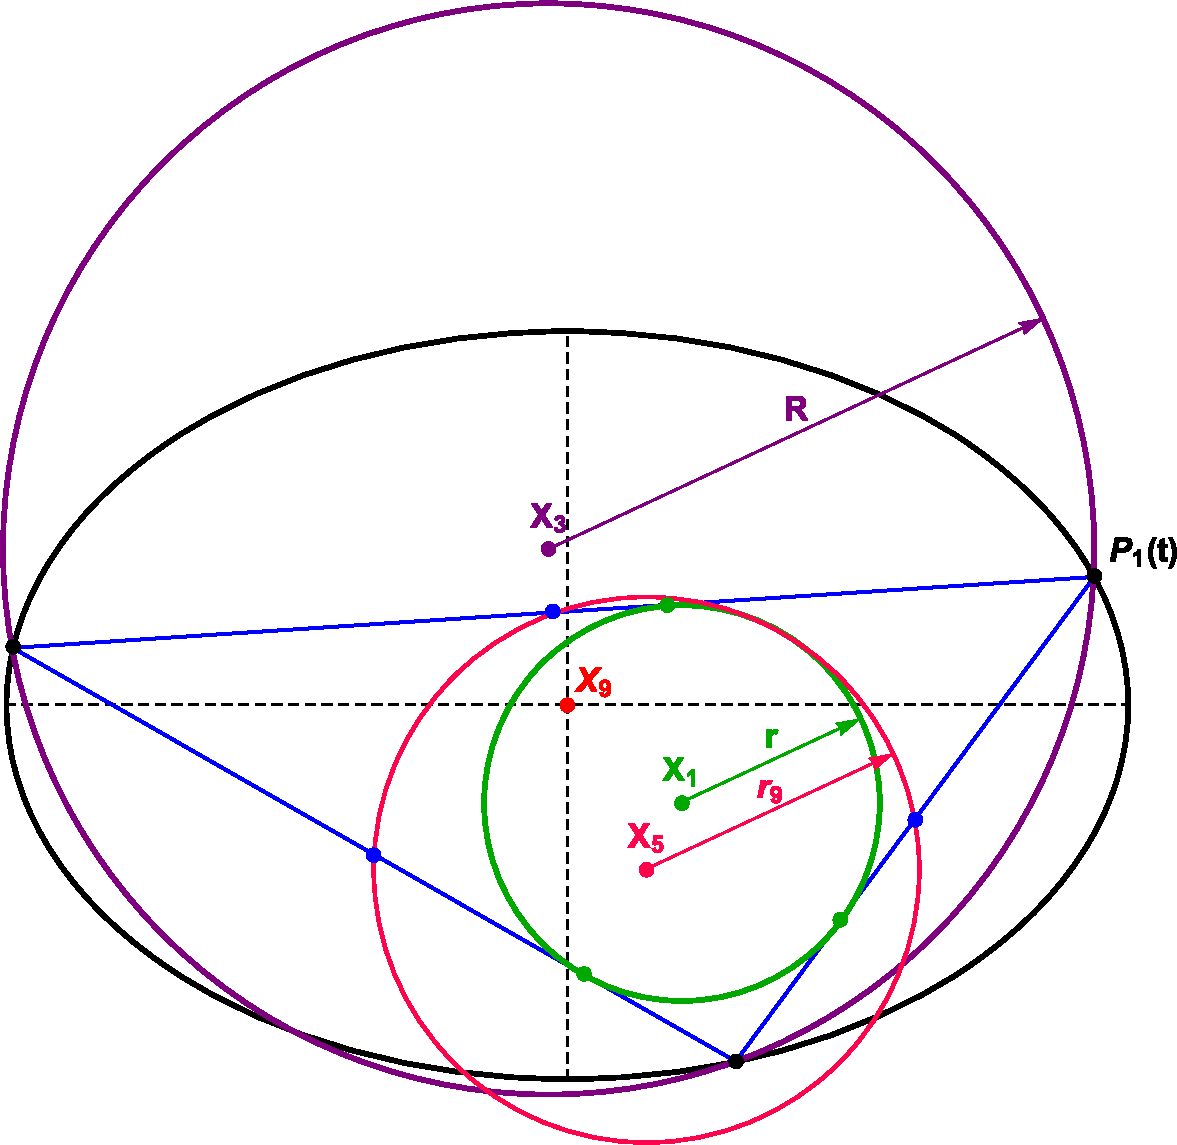
\includegraphics[width=.8\textheight]{pics/0070_Radii.pdf}
\end{figure}
\end{frame}

\begin{frame}{Plotting Radii}
\begin{figure}
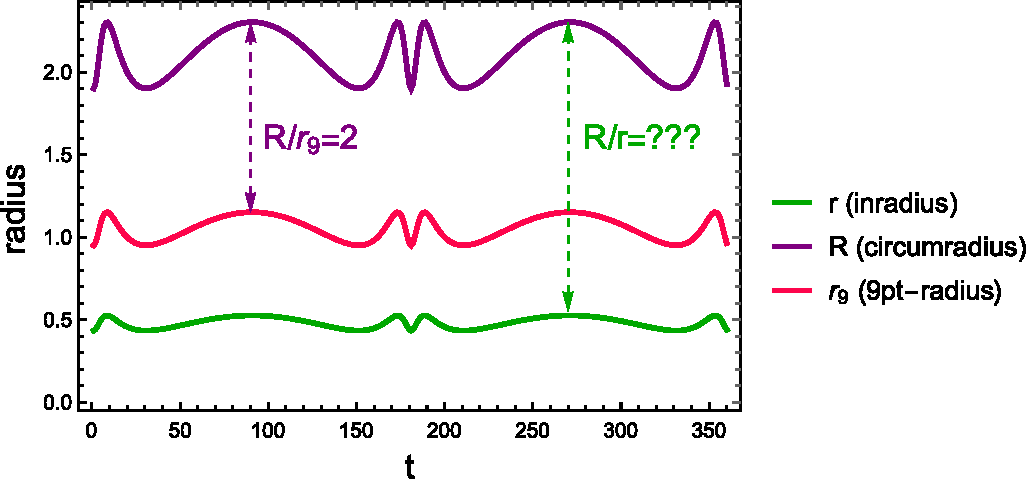
\includegraphics[height=.7\textheight]{pics/0075_radii_plot.pdf}
\end{figure}
\end{frame}

\begin{frame}{A New Constant of Motion!}

\begin{figure}
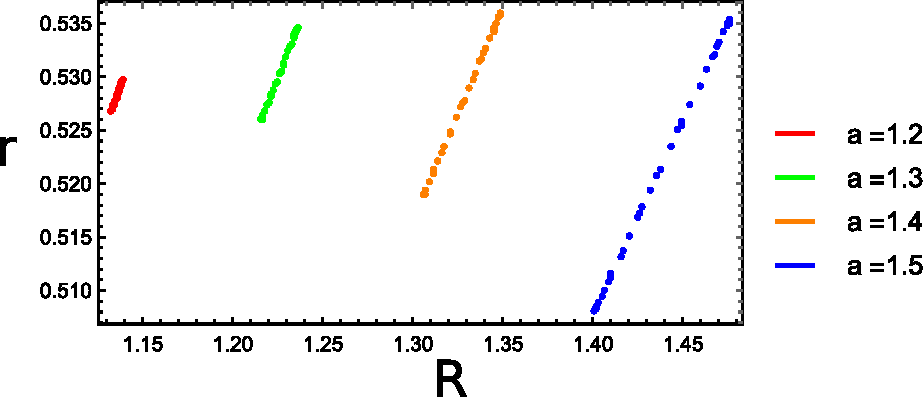
\includegraphics[height=.5\textheight]{pics/0080_radii_scatter.pdf}
\end{figure}
\begin{center}
\boxed{\frac{r}{R}=\gamma\,L-4}    
\end{center}
\end{frame}



\section{Three Amazing Corollaries}
\frame{\sectionpage}
\begin{frame}{Sum of Orbit Cosines is Conserved!}
\begin{equation*}
\sum_{i=1}^{3}{\cos\theta_i}=1+\frac{r}{R}=\gamma{L}-3
\end{equation*}

\begin{figure}
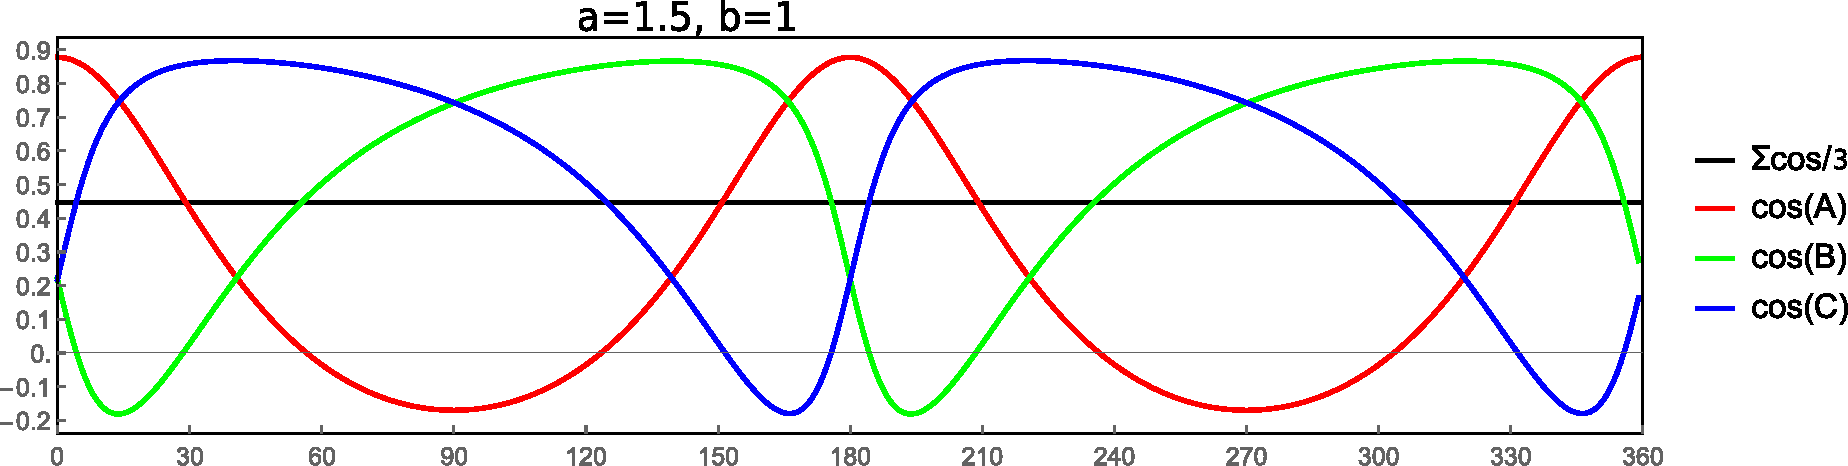
\includegraphics[width=.8\textwidth]{pics/0090_cosine_sum_n3.pdf}
\end{figure}
\end{frame}

\begin{frame}{Product of Excentral Cosines is Conserved!  \href{https://youtu.be/P8ykpE_ZbZ8}{[video]}}
\begin{tabular}{rl}
\begin{tabular}{r}
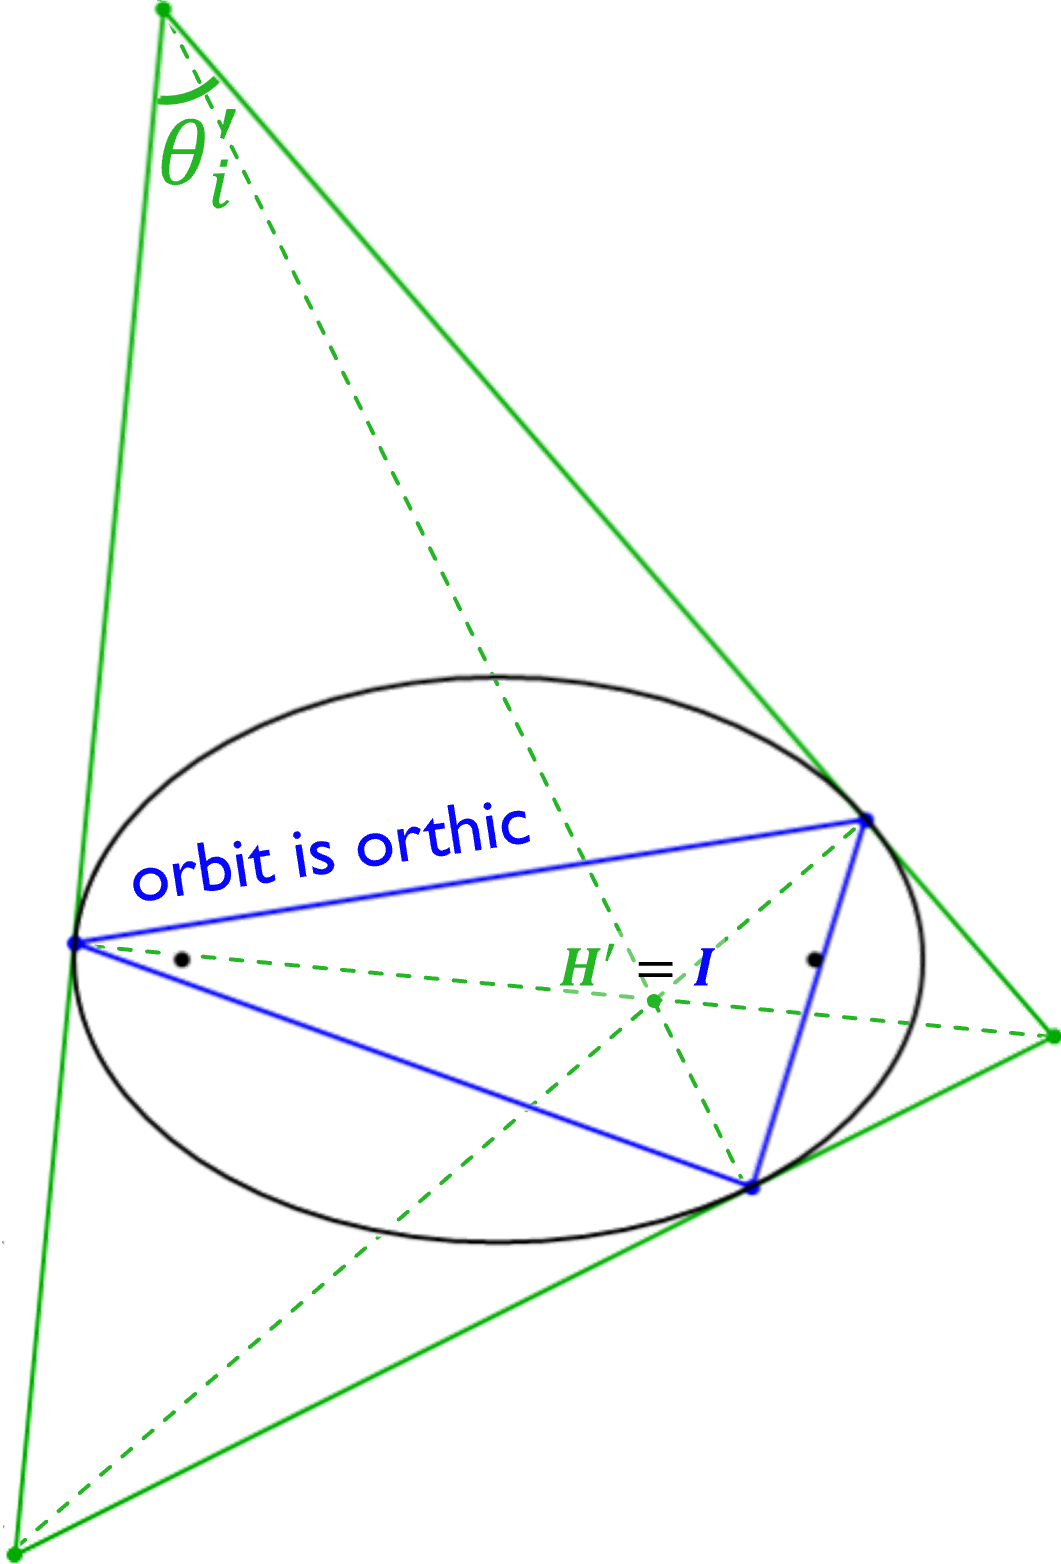
\includegraphics[height=.7\textheight]{pics/0076_product_of_excentral.png}
\end{tabular} & \begin{tabular}{l}
\parbox{0.5\linewidth}{
  \begin{minipage}{0.45\textwidth} $$\prod_{i=1}^{3}{|\cos\theta_i'|}=\frac{1}{4}\frac{r_h}{R_h}=\frac{\gamma{L}}{4}-1$$ \end{minipage}}
\end{tabular}  \\
\end{tabular}
\end{frame}

\begin{frame}{Orbit-to-Excentral Area Ratio is Conserved!}
\begin{tabular}{rl}
\begin{tabular}{r}
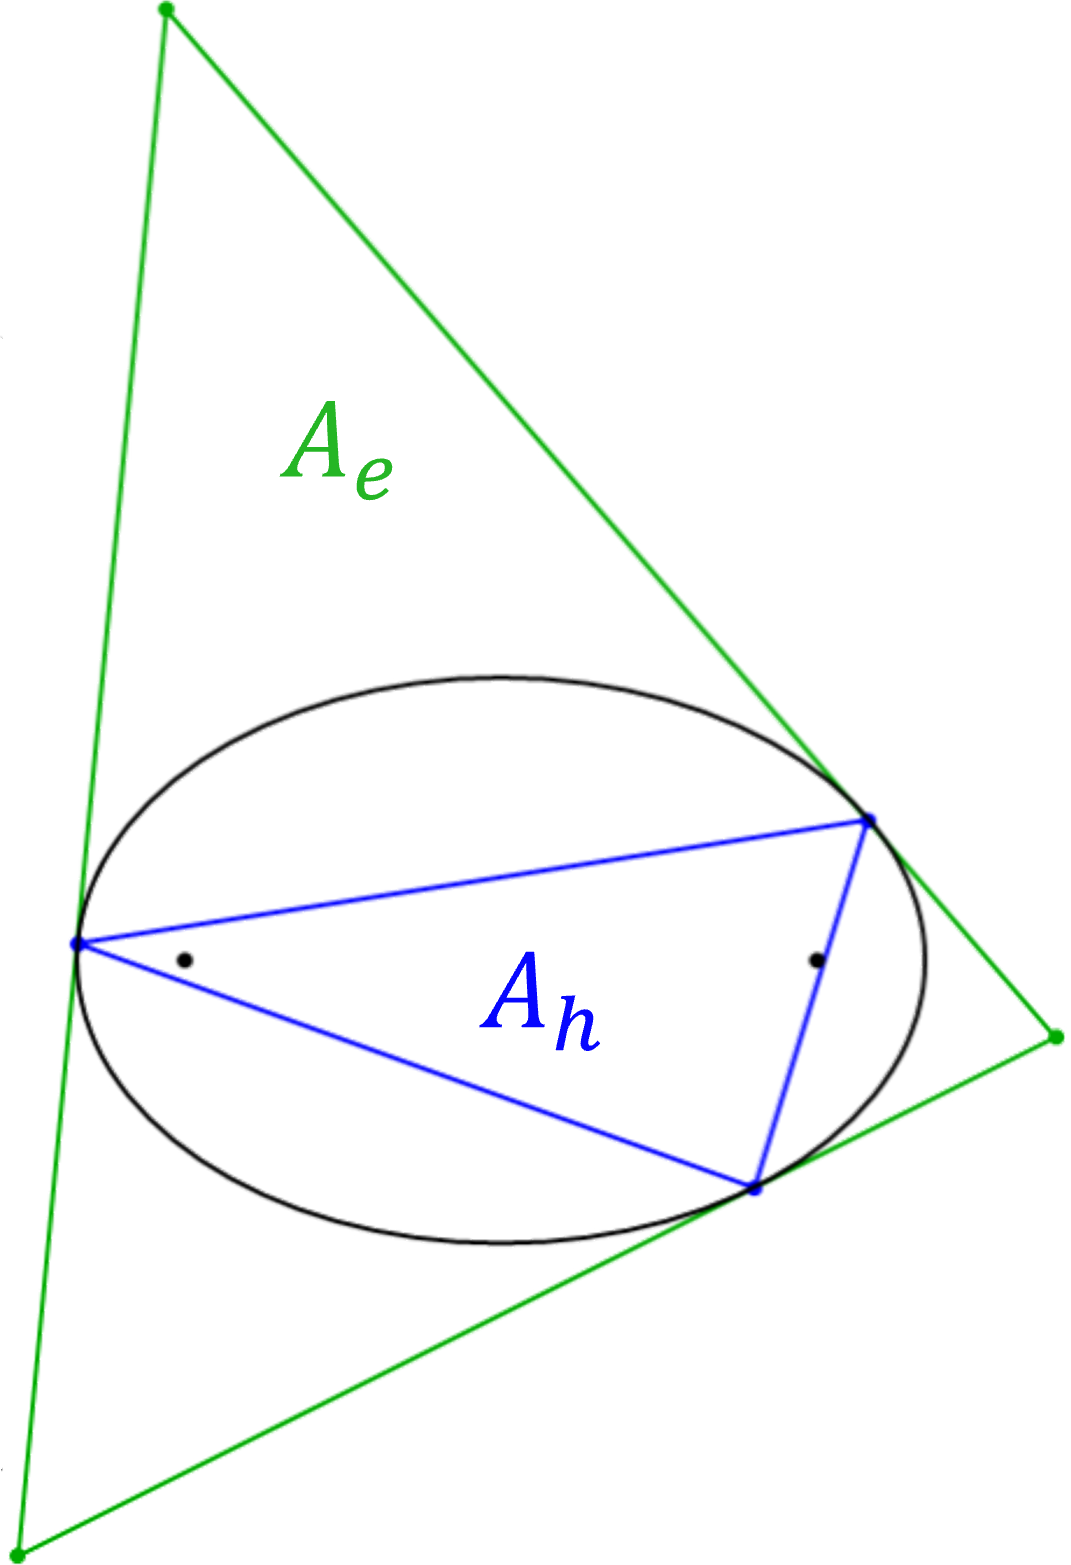
\includegraphics[height=.7\textheight]{pics/0077_area_ratio.png}
\end{tabular} & \begin{tabular}{l}
\parbox{0.5\linewidth}{
  \begin{minipage}{0.45\textwidth} $$\frac{A_h}{A_e}=\frac{1}{2}\frac{r_h}{R_h}$$ \end{minipage}}
\end{tabular}  \\
\end{tabular}
\end{frame}

\section{Generalize $\forall{N}$}
\frame{\sectionpage}
\begin{frame}{Monge's Orthoptic Circle \href{https://youtu.be/9fI3iM2jrmI}{[video]}}
\begin{tabular}{cl}
\begin{tabular}{c}
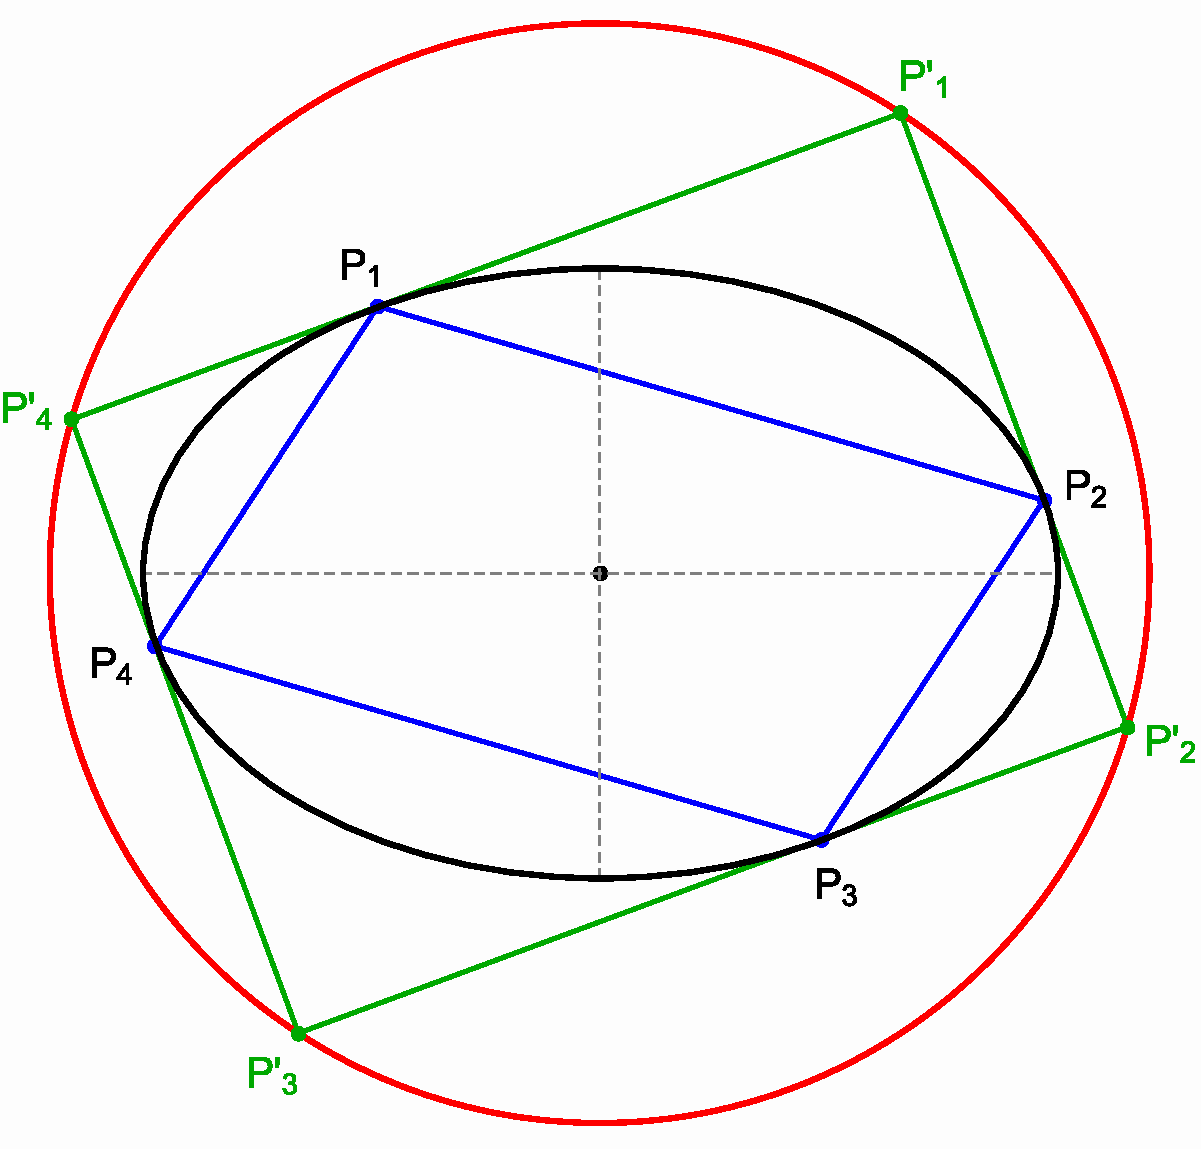
\includegraphics[height=.8\textheight]{pics/0200_monge_orthoptic.pdf}
\end{tabular} & \begin{tabular}{l}
\parbox{0.5\linewidth}{
  \begin{minipage}{0.5\textwidth}
 \begin{itemize}
    \item * Stationary Circle
    \item * Rectangle diagonals.
    \item * $\sum{\cos{\theta_i}}=0$.
    \item * $\prod{\cos{\theta_i'}}=0$.
\end{itemize}
\end{minipage}}
\end{tabular}  \\
\end{tabular}
\end{frame}

\begin{frame}{Generalized Stationary Circle     \href{https://youtu.be/dINE4aH1cvk}{[video 1]} and \href{https://youtu.be/EFeINGIDFrg}{[video 2]}}
\begin{figure}
    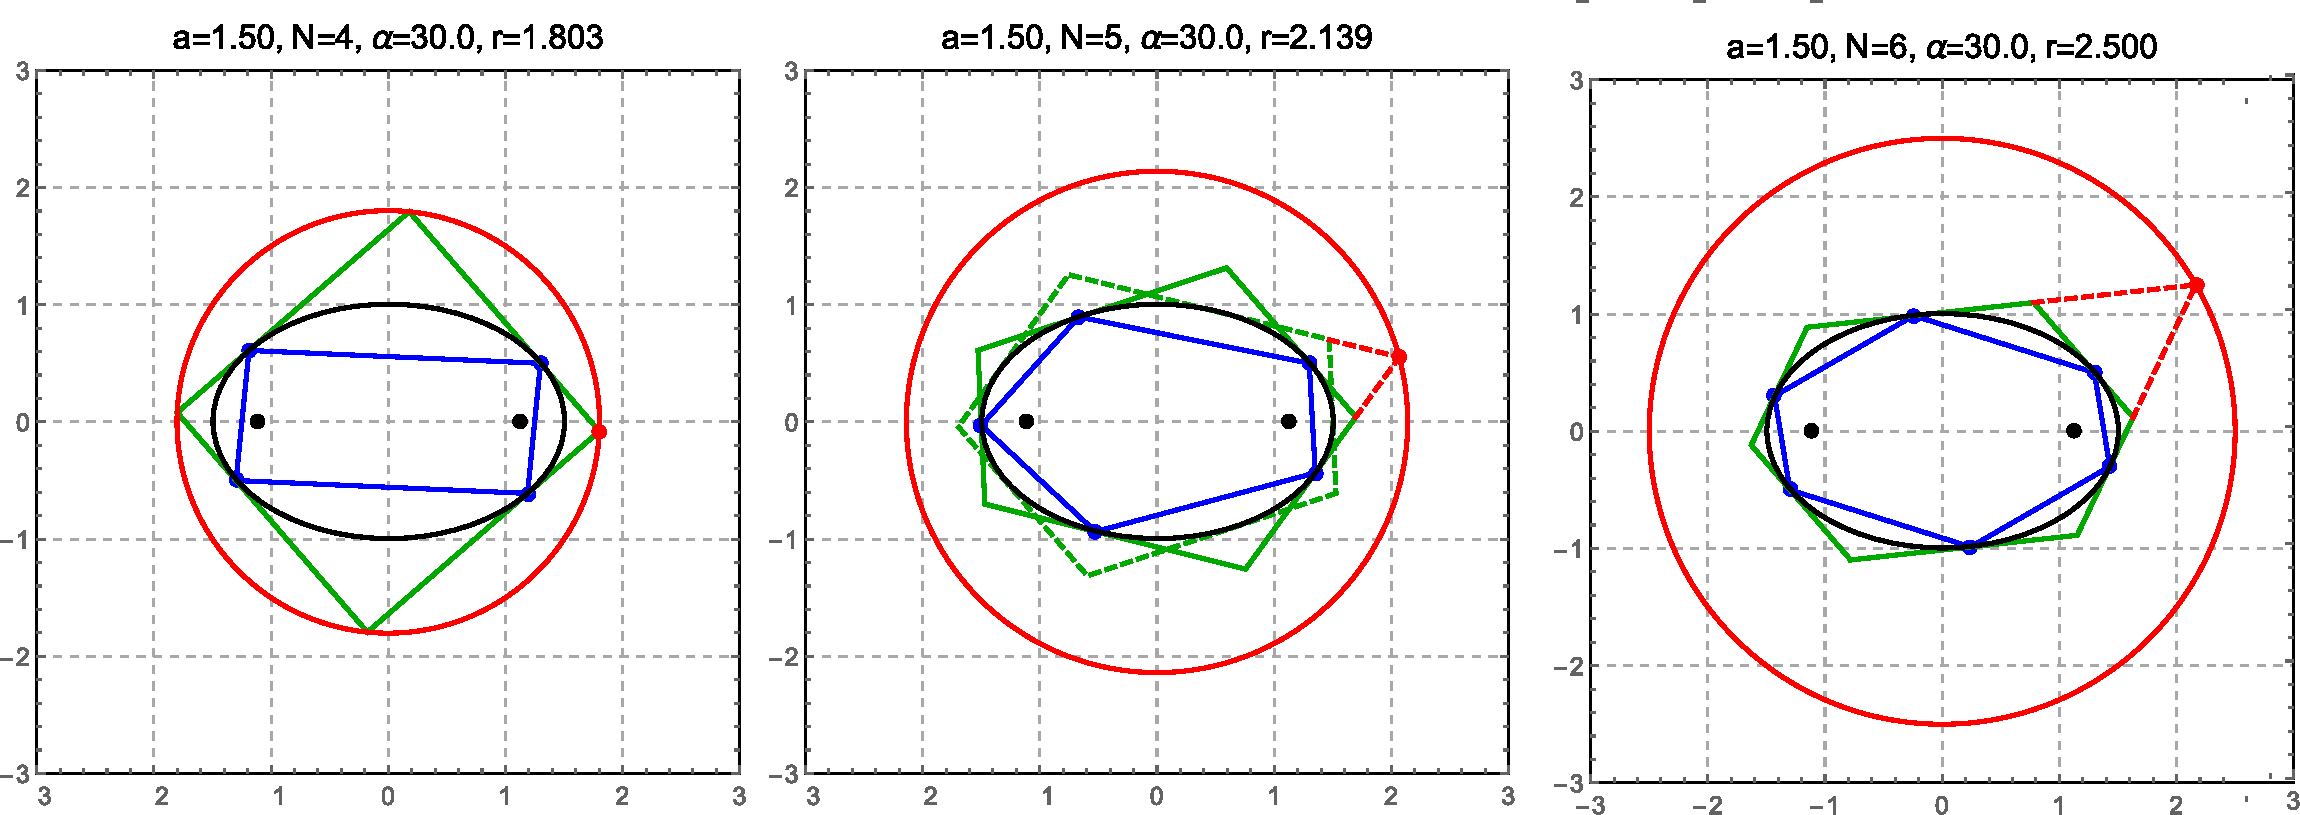
\includegraphics[clip,trim={0 0 0 1.66cm},width=\textwidth]{pics/0180_circ_grid_v3.pdf}
\end{figure}
\vspace*{-.125cm}
$\implies E\,'_{i}\cap-E\,'_{i+1}$ is a stationary circle of  $r^*=1/\gamma$
\end{frame}

\begin{frame}{$N>3$ Mittenpunkt \href{https://youtu.be/TV2p7fPlYfE}{[video 1]} and Extouchpoints \href{https://youtu.be/Bpc-MrR2IMc}{[video 2]}}
\begin{figure}
    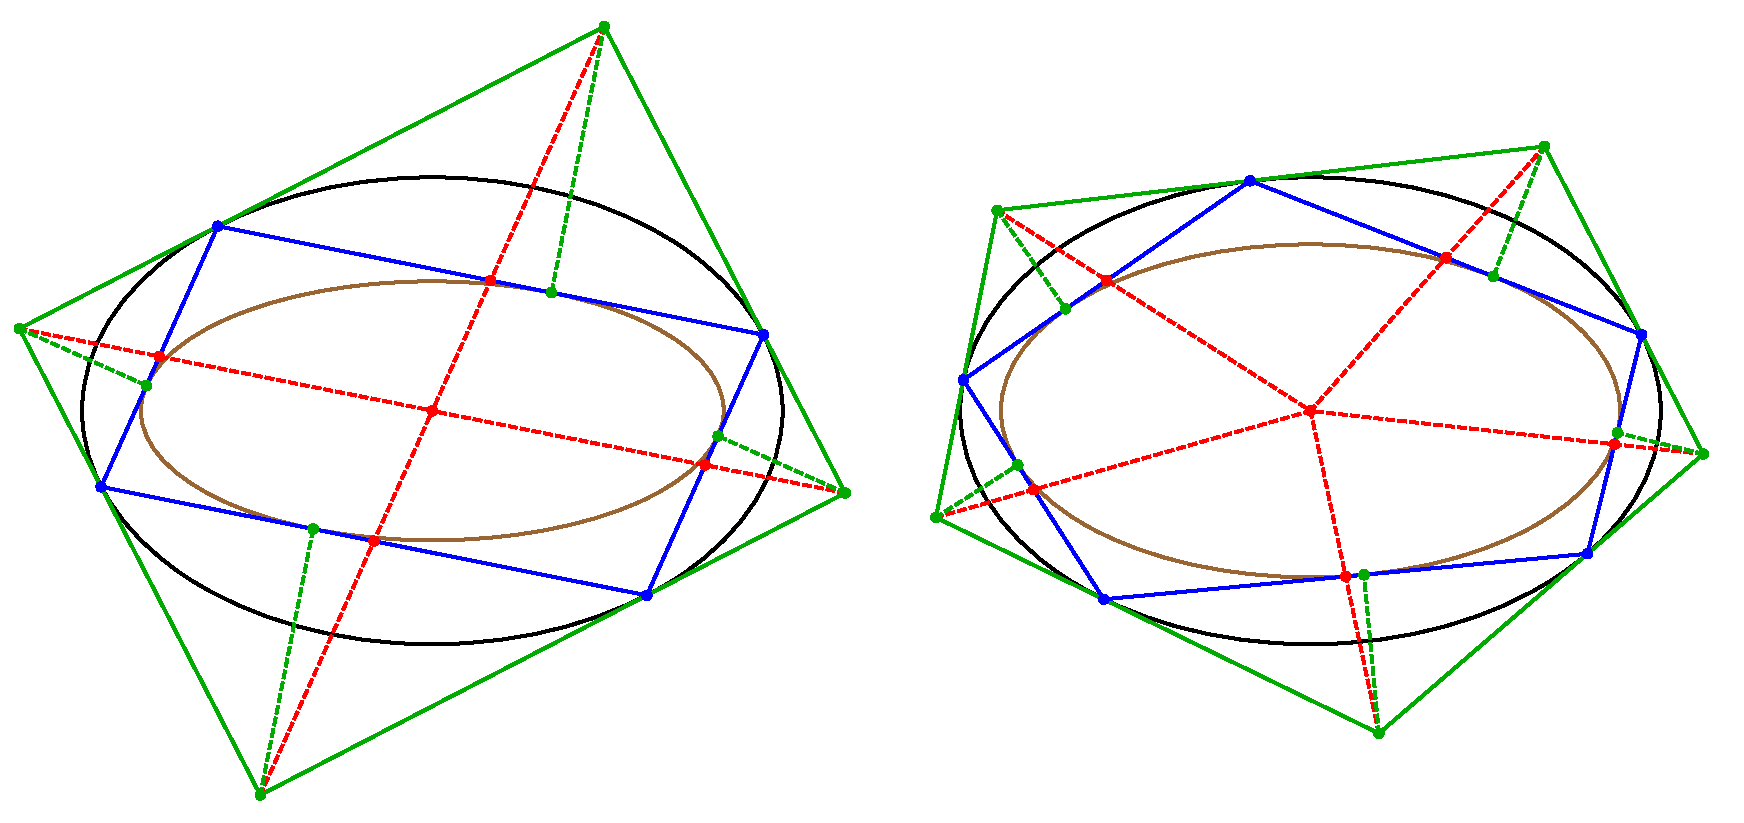
\includegraphics[width=\textwidth]{pics/0165_extouch.pdf}
    \label{fig:gen-mitten}
\end{figure}
\end{frame}

\begin{frame}{Cosine Sums for $N>3$}
\begin{figure}
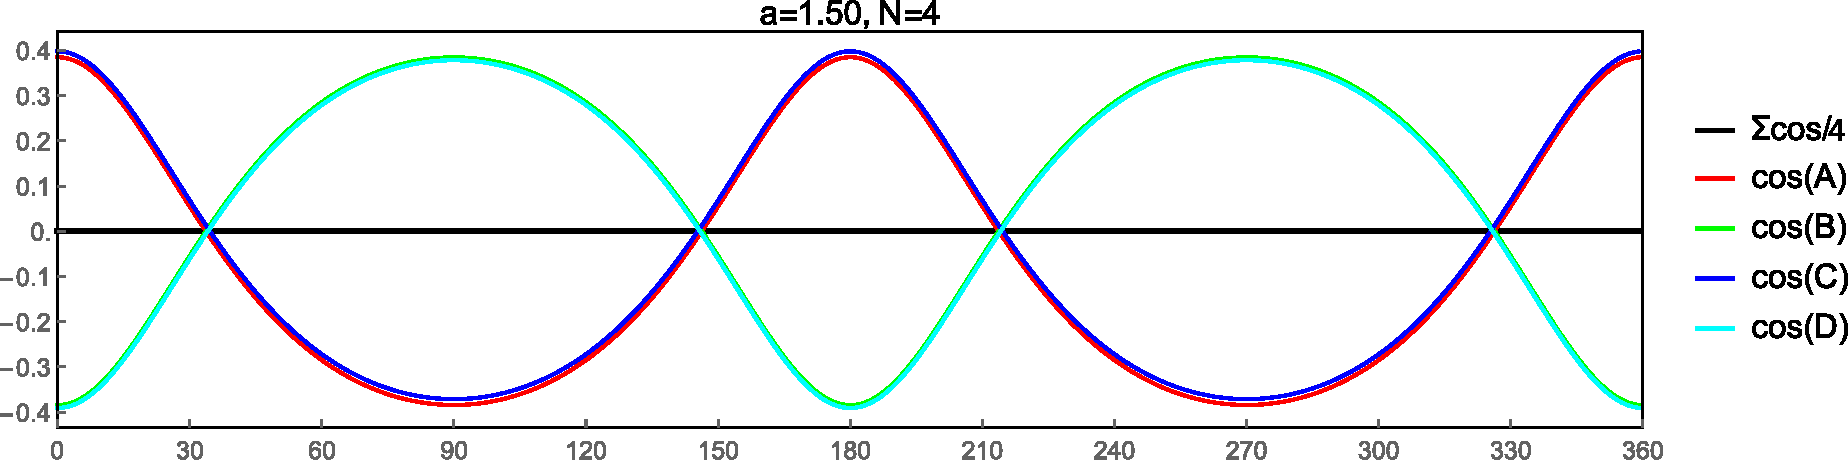
\includegraphics[width=.9\textwidth]{pics/0091_cosine_sum_n4.pdf}\\
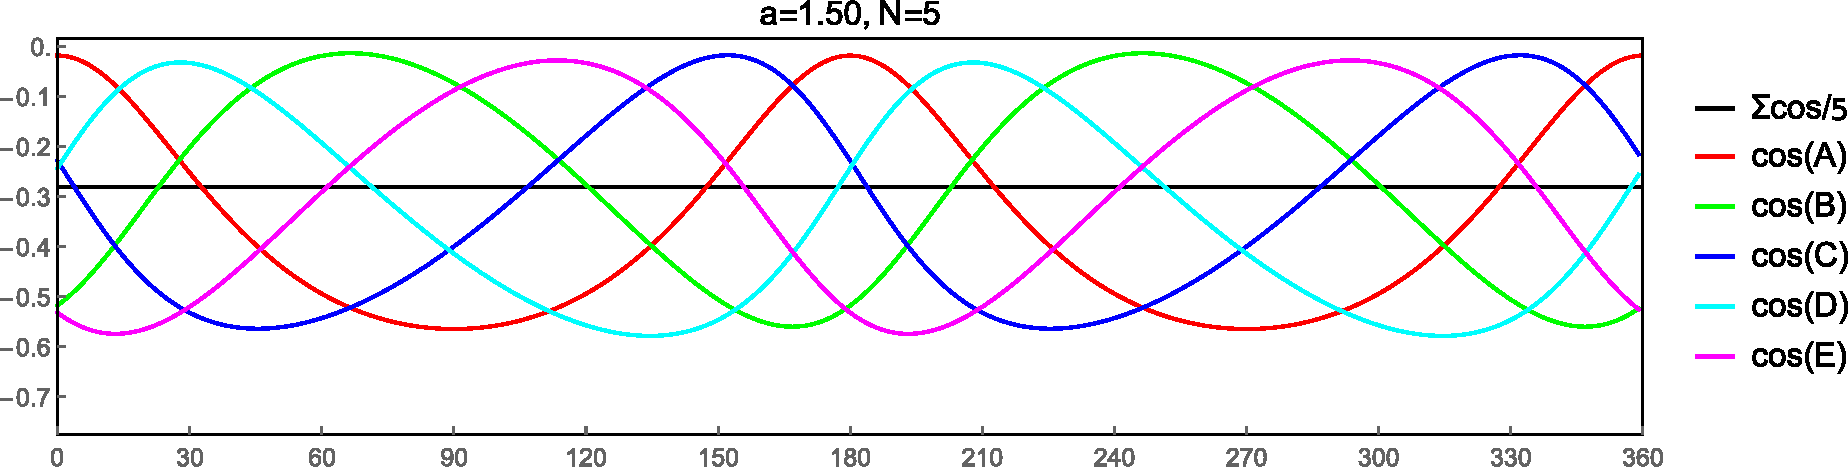
\includegraphics[width=.9\textwidth]{pics/0092_cosine_sum_n5.pdf}
\end{figure}
\end{frame}

\begin{frame}{Sum, Product, Area Ratios are Conserved!}
\begin{tabular}{cl}
\begin{tabular}{c}
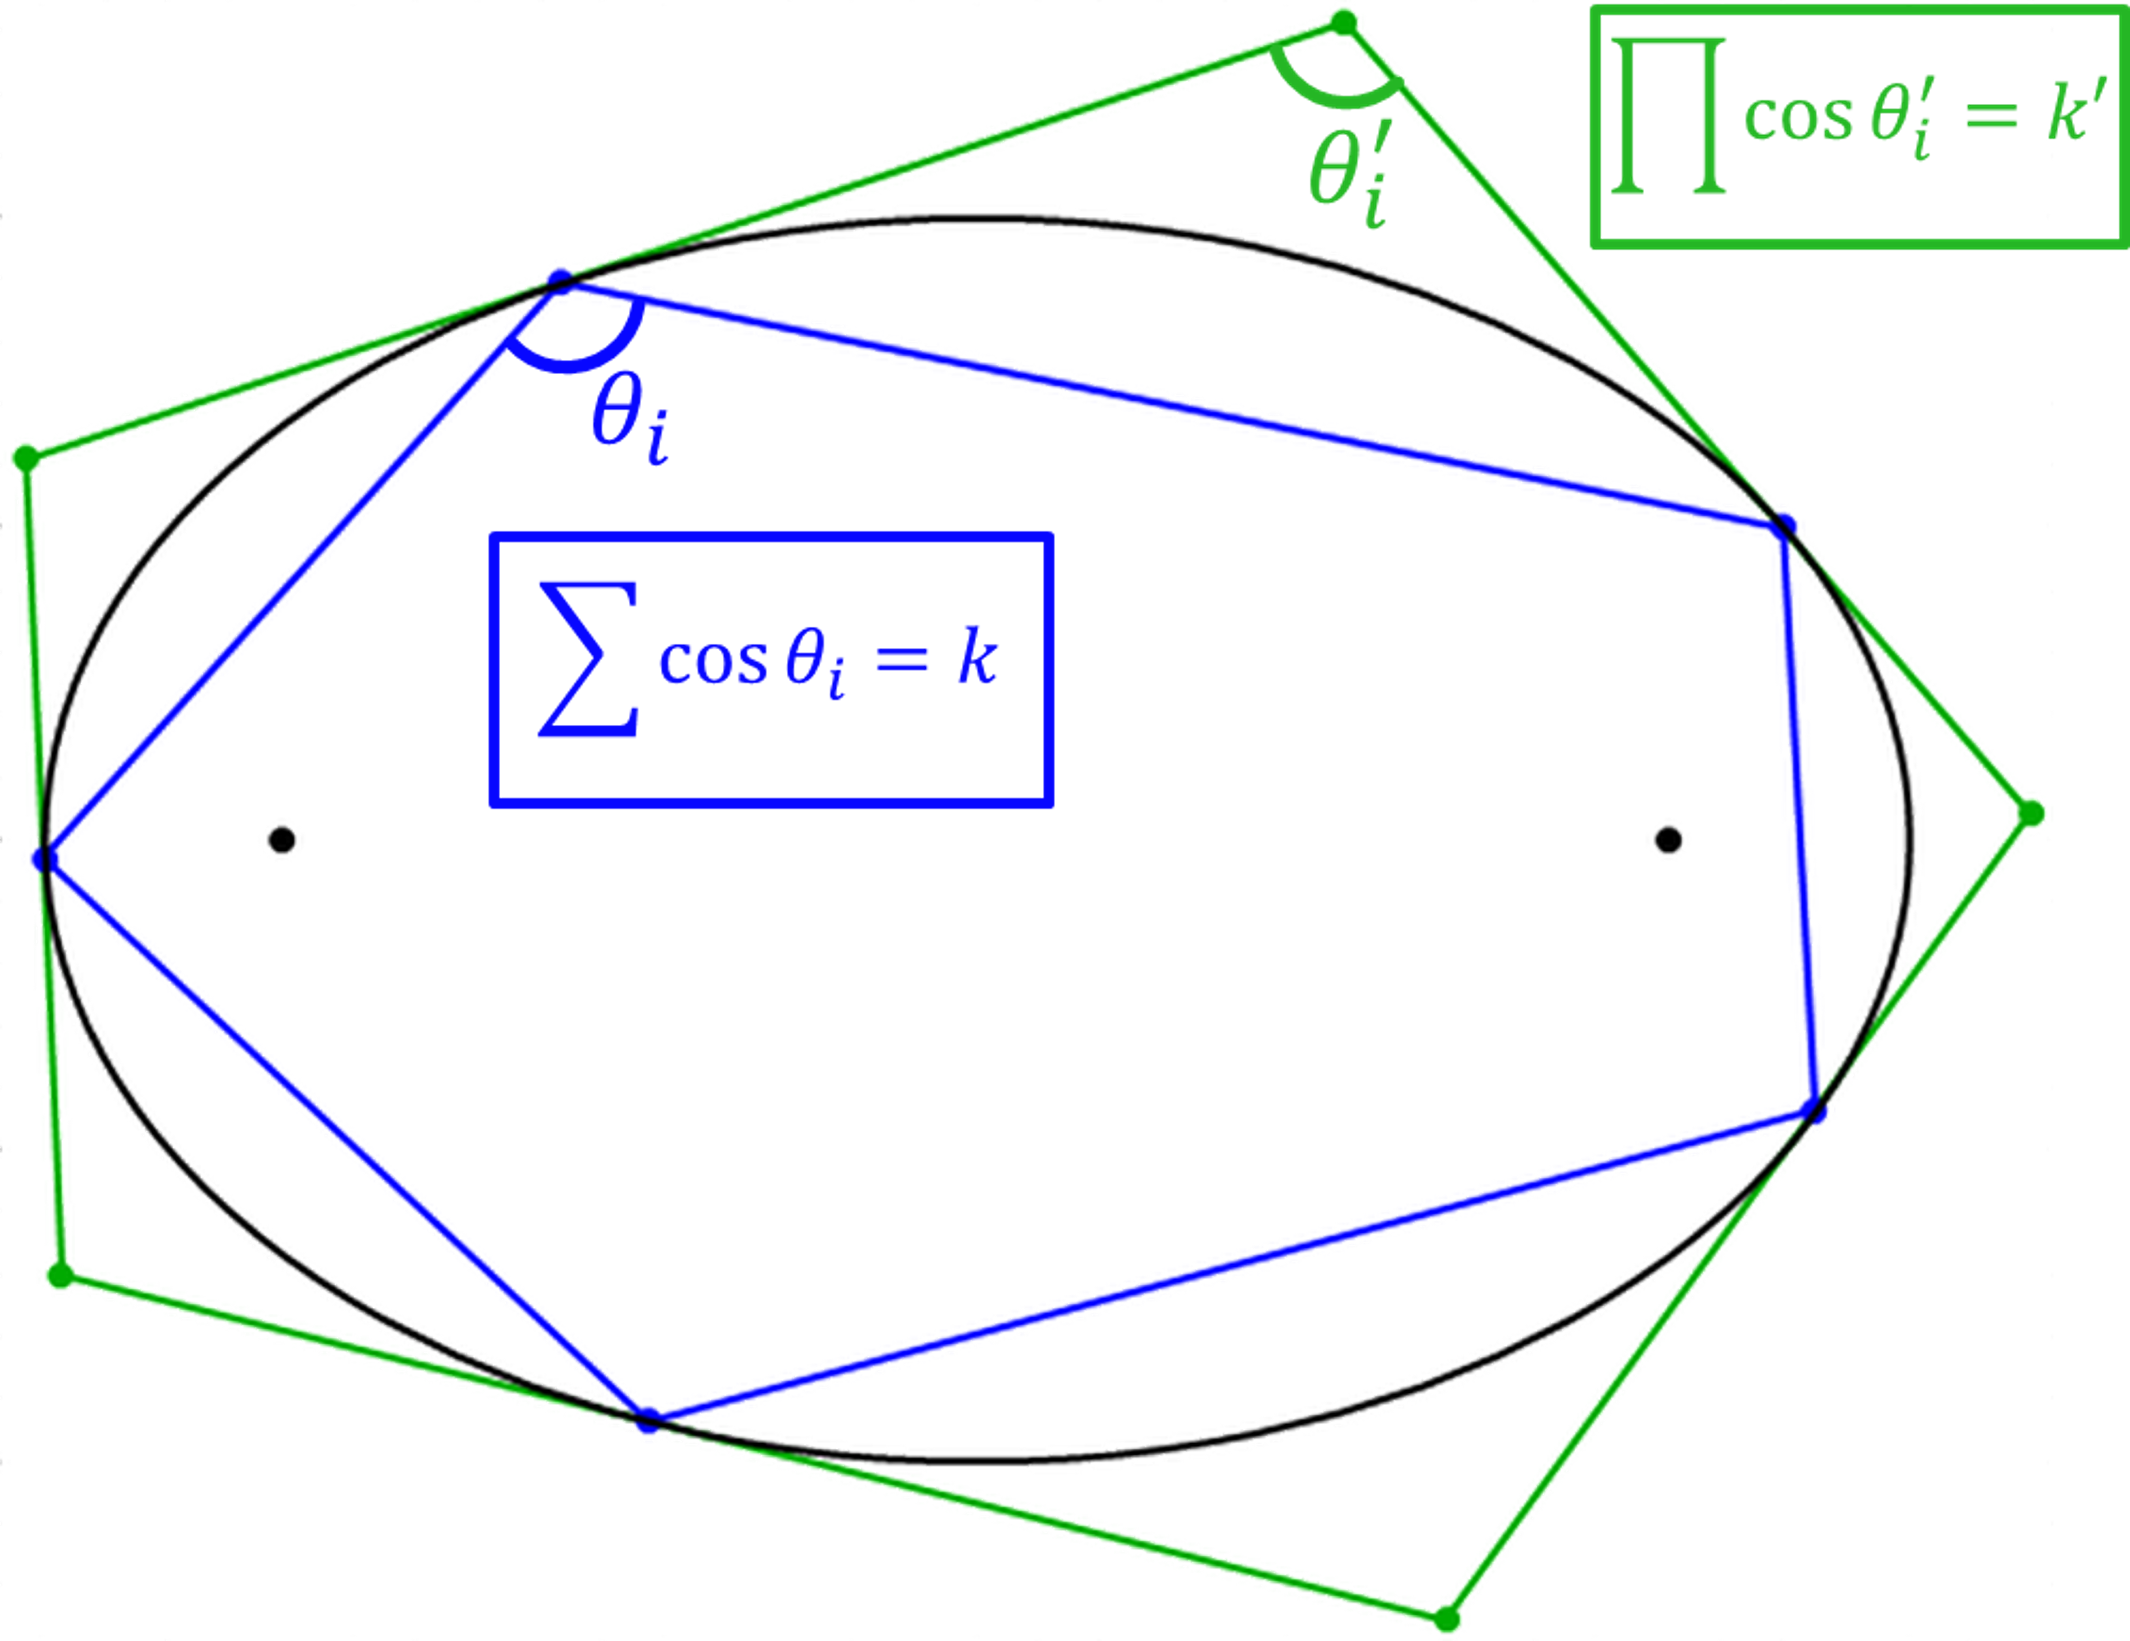
\includegraphics[height=.6\textheight]{pics/0078_cosine_sum_and_product_for_all_n.png}
\end{tabular} & \begin{tabular}{l}
\parbox{0.5\linewidth}{
  \begin{minipage}{0.5\textwidth}
\begin{itemize}
\item $\implies$ $\sum_{i=1}^{N}{\cos{\theta_i}}$ conserved  $\forall{N}$.
\item $\implies$ $\prod_{i=1}^{N}{\cos{\theta_i'}}$ conserved  $\forall{N}$.
\item $\implies$ $A'/A$ conserved $\forall{N}$ \textbf{odd}.
\end{itemize}
\end{minipage}}
\end{tabular}  \\
\end{tabular}
\end{frame}

\section{Conclusion \& Questions}
\begin{frame}{Summary}
\begin{figure}
    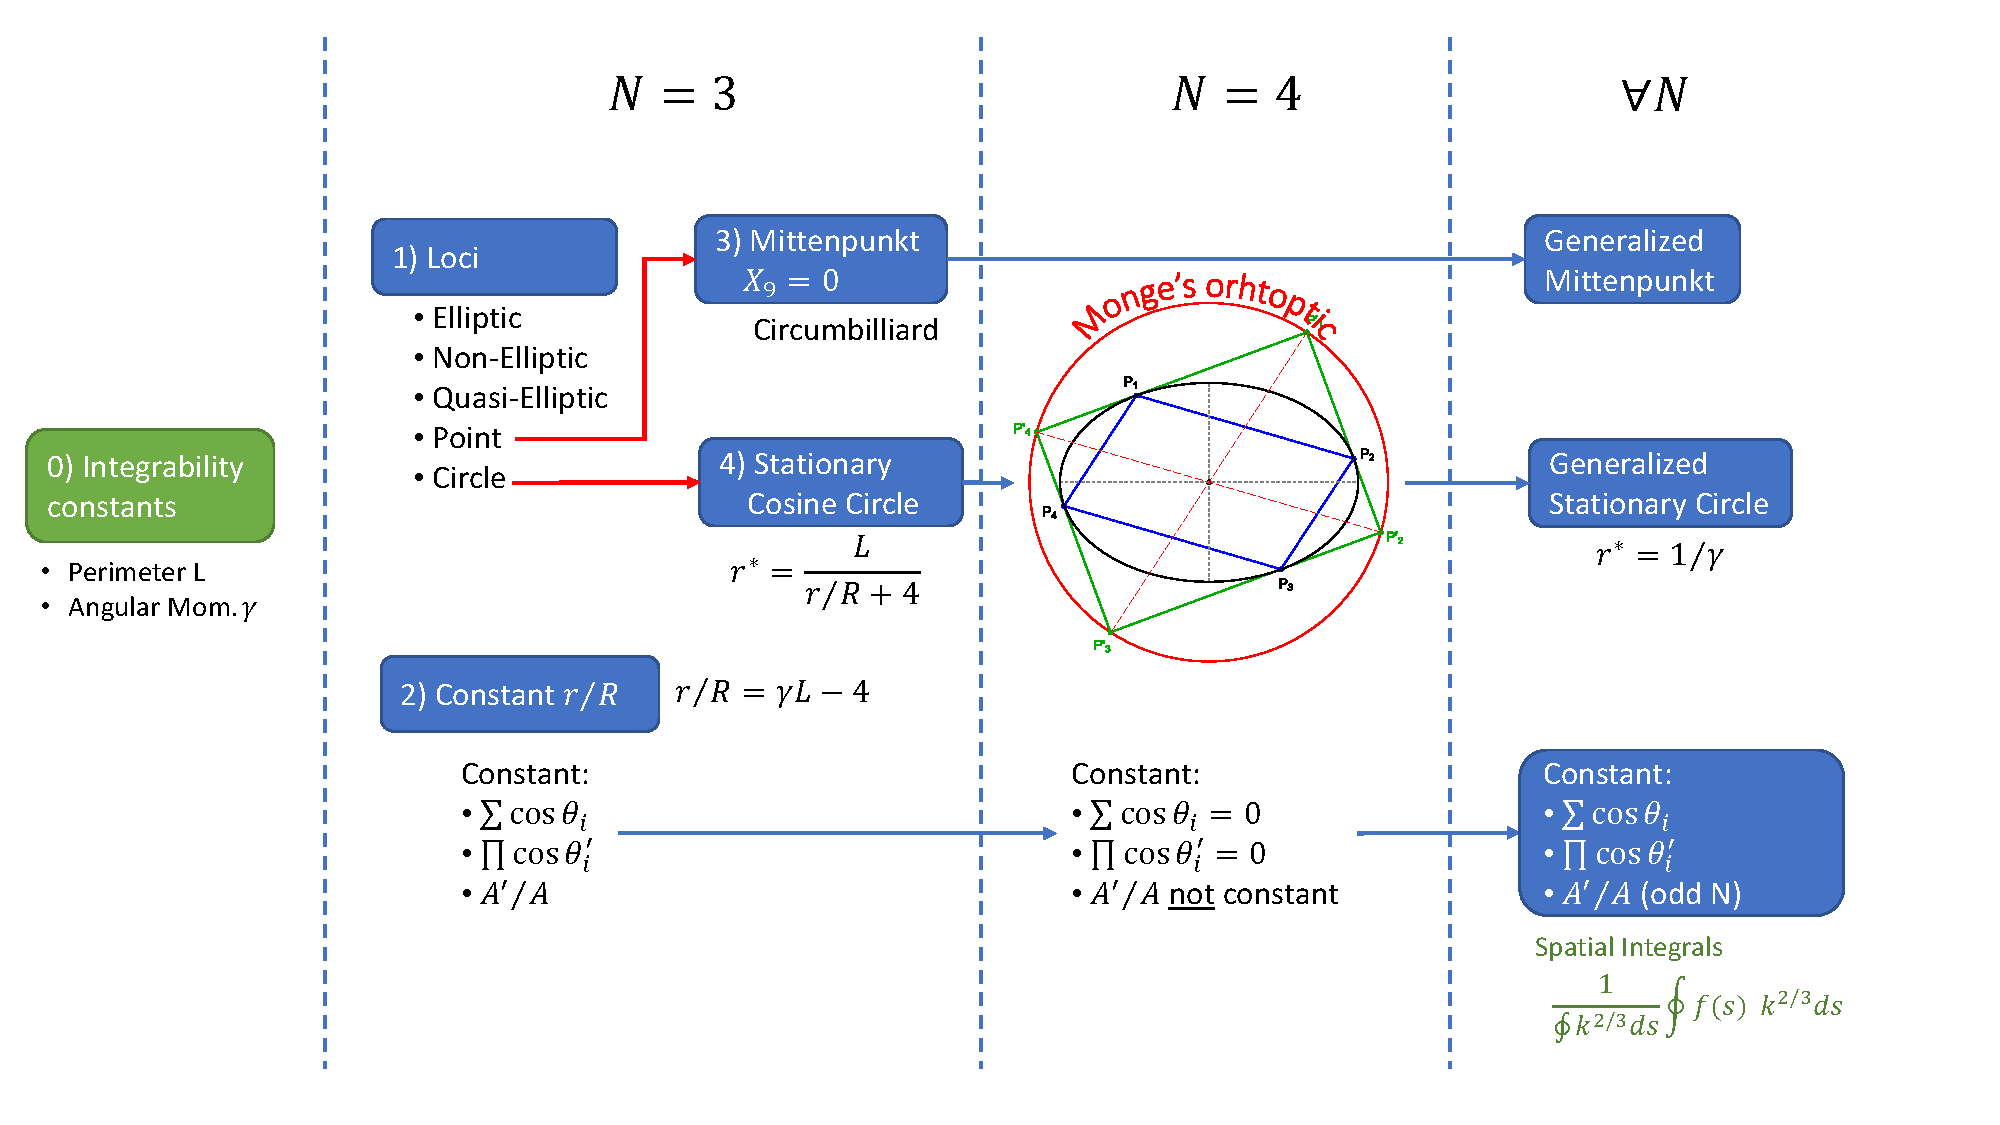
\includegraphics[clip,trim={0 0 0 0},height=.9\textheight]{pics/0002_diagram_slide.pdf}
\end{figure}
\end{frame}

\begin{frame}{Project's \href{https://dan-reznik.github.io/Elliptical-Billiards-Triangular-Orbits/}{[Homepage]}}
\begin{figure}
    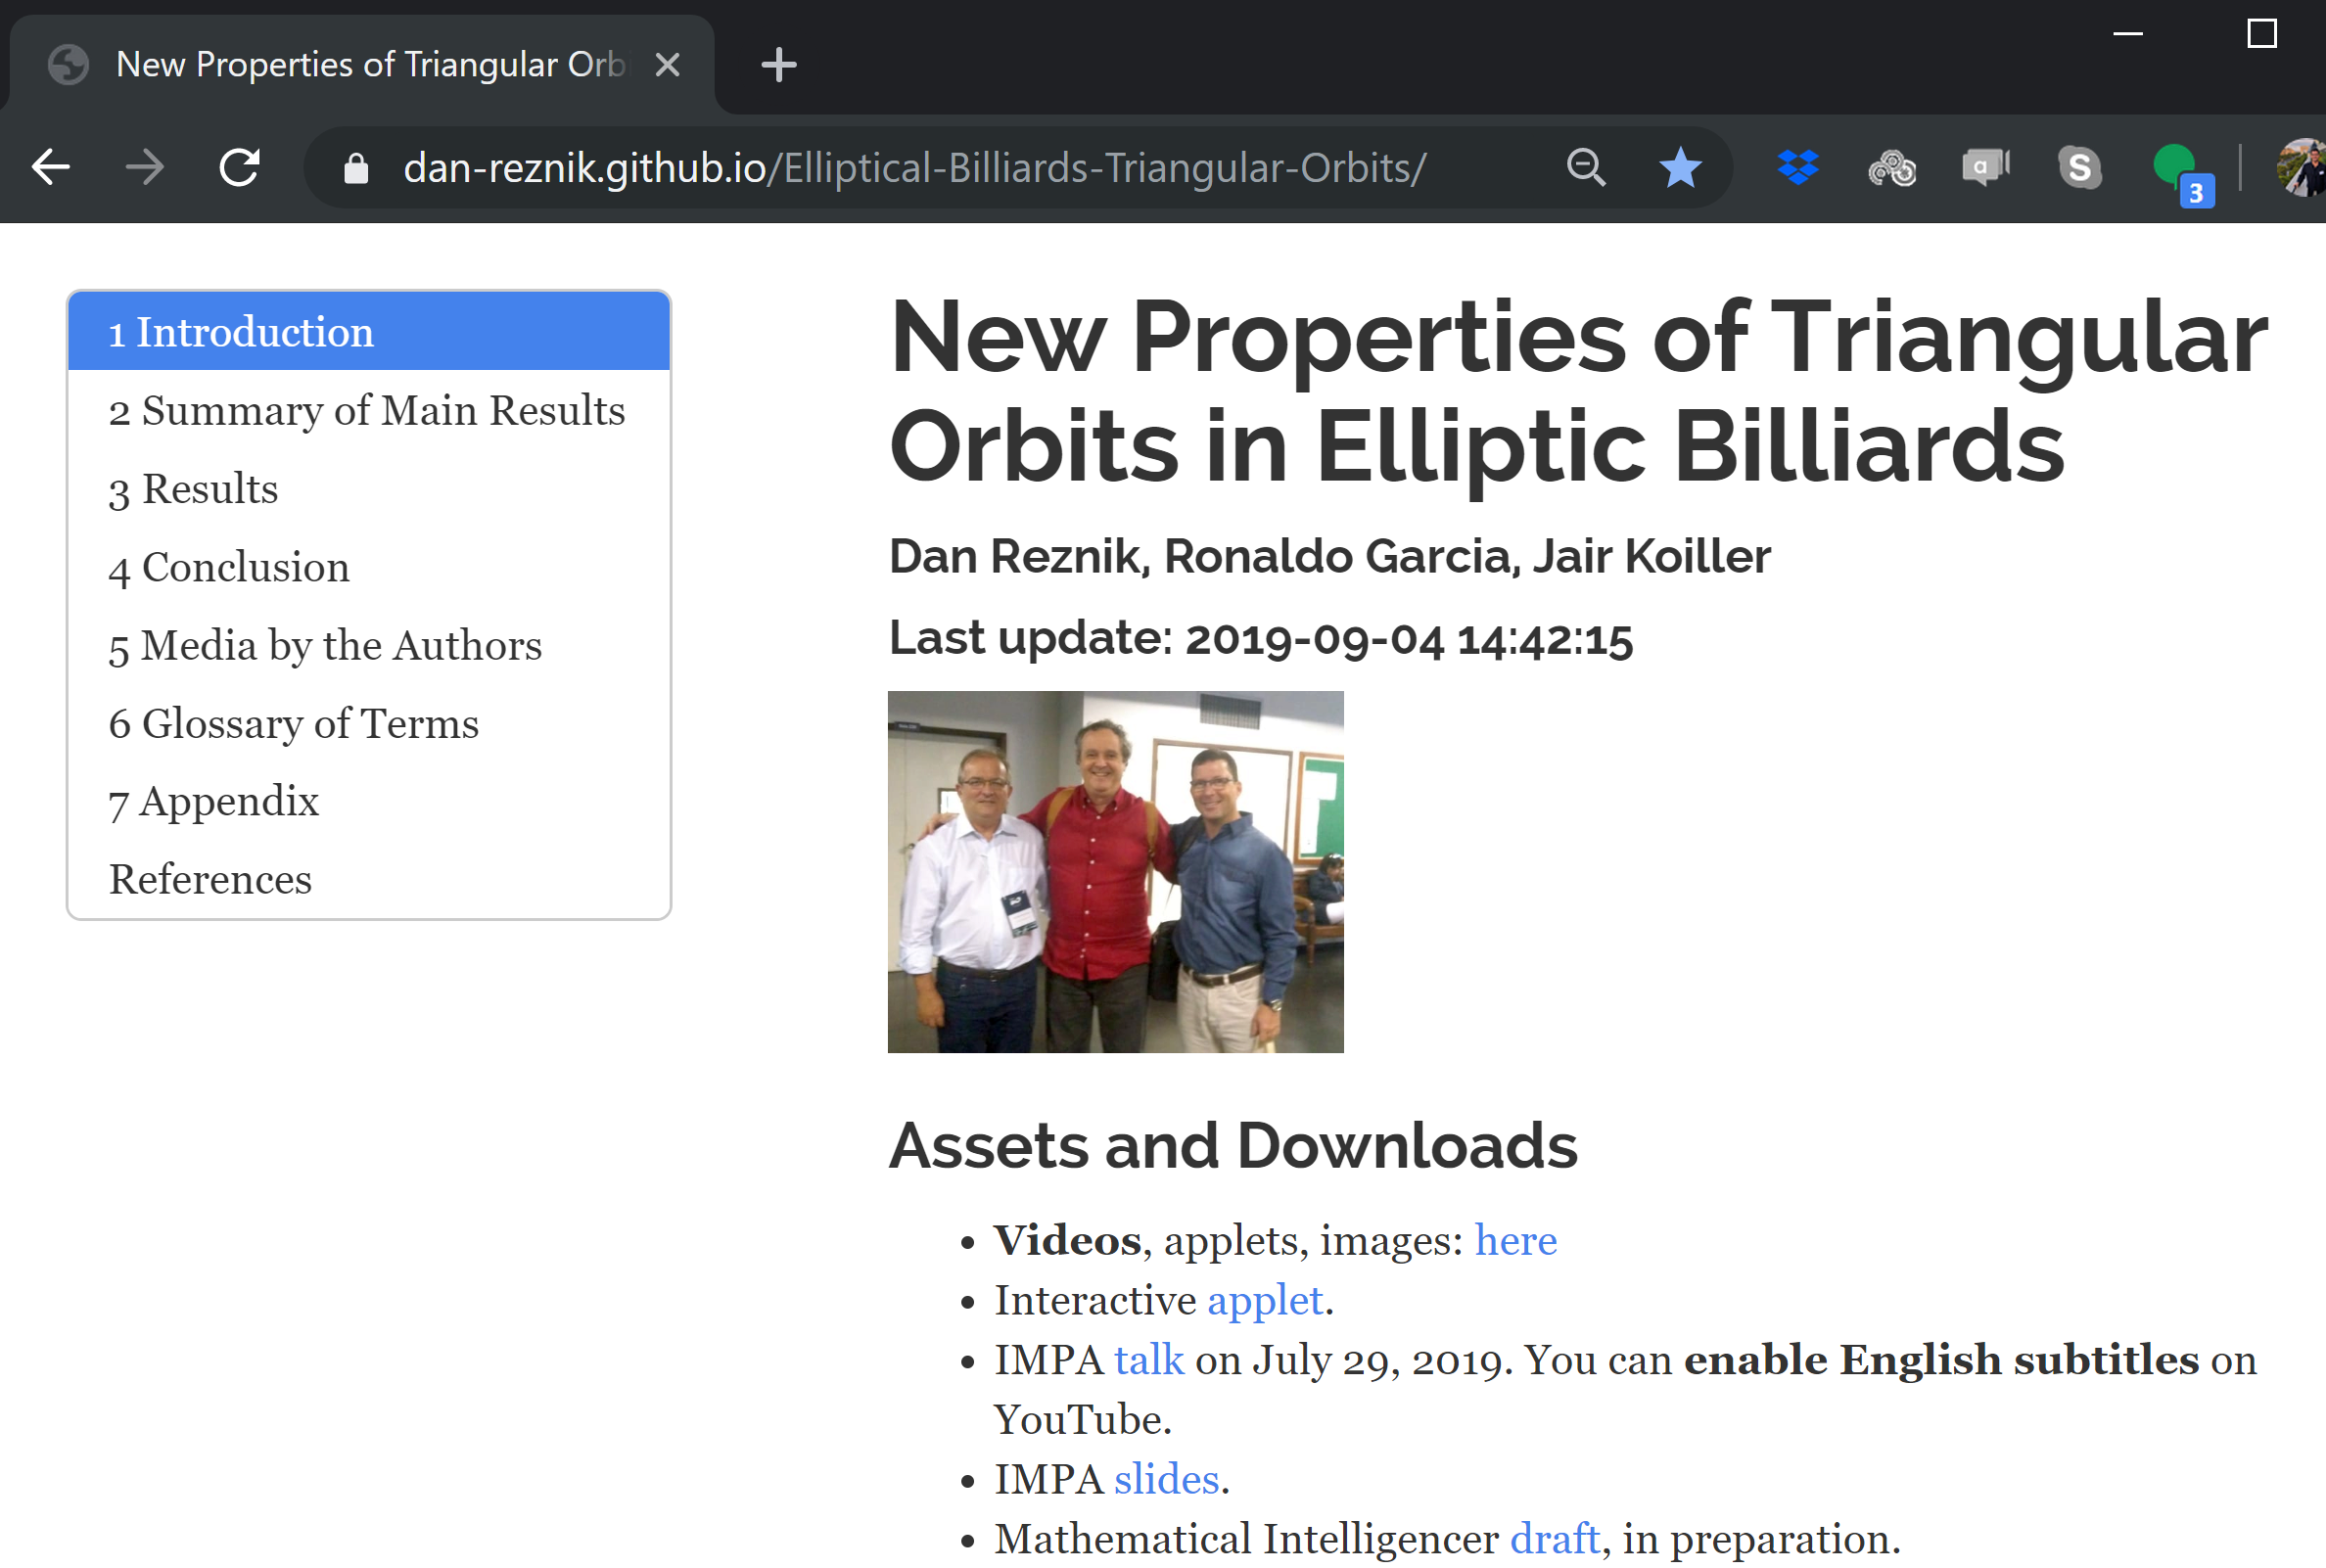
\includegraphics[height=.8\textheight]{pics/0000_website.png}
\end{figure}

\end{frame}

\begin{frame}{Questions}
\begin{itemize}
    \item * $N=3$: why is a locus is elliptic or non?
    \item * Invariants for Ellipsoidal (3d) Billiard?
    \item * Invariants in self-intersecting orbits? (\href{https://youtu.be/cCYxN7ueGV4}{N=4} and \href{https://youtu.be/ECe4DptduJY}{N=5})
    \item * Invariants in non-billiard (Poncelet) orbit families?
    \item * Invariants for orbits on sphere?
\end{itemize}

\vspace*{1cm}

\begin{minipage}{.2\textwidth}
\textbf{Thanks!}
\end{minipage}
\begin{minipage}{.3\textwidth}
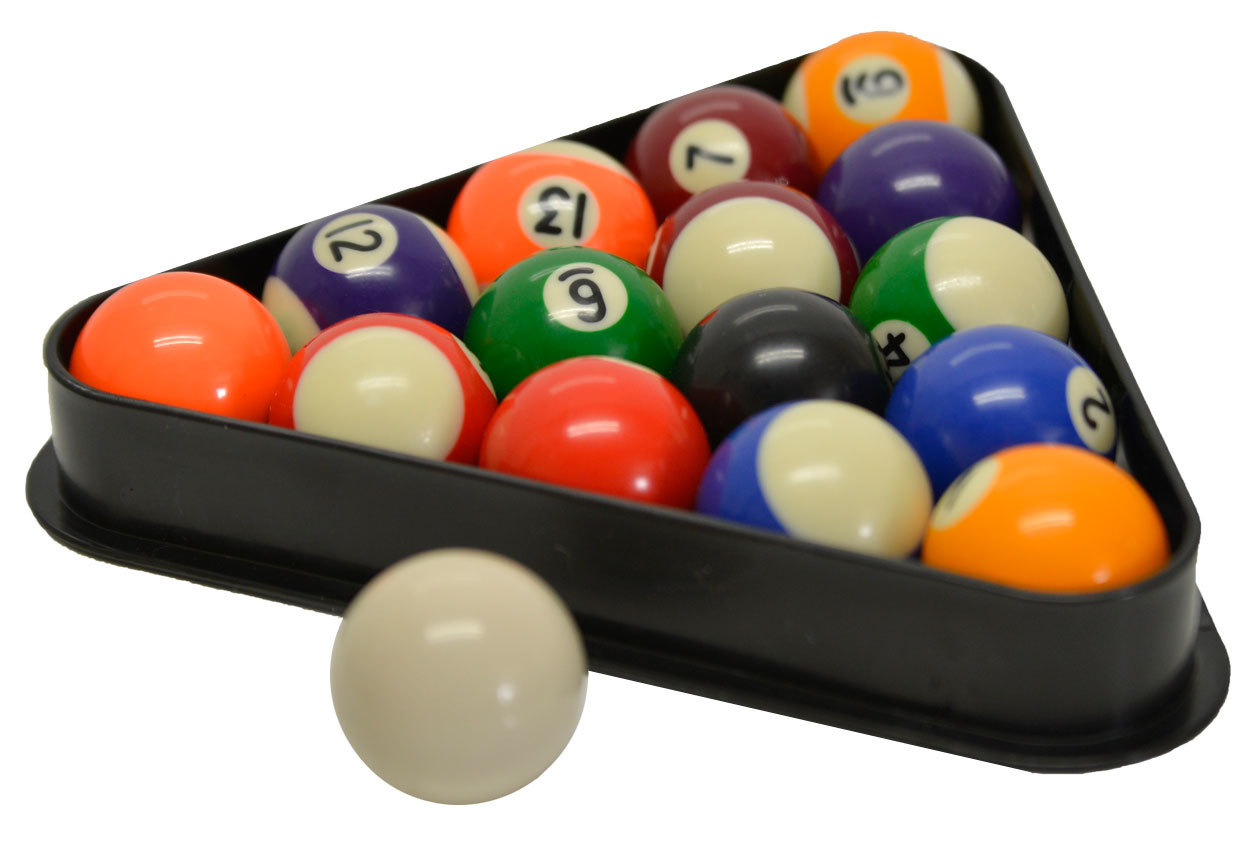
\includegraphics[height=0.25\textheight]{pics/0000_billiard_rack.png} 
\end{minipage}
\begin{minipage}{.4\textwidth}
\href{dreznik@gmail.com}{dreznik[@]gmail[.]com}\\
\href{ragarcia@ufg.br}{ragarcia[@]ufg[.]br}\\
\href{jairkoiller@gmail.com}{jairkoiller[@]gmail[.]com}
\end{minipage}
\end{frame}



\end{document}